% !BIB program = bibtex
\documentclass{article}

\usepackage{graphicx, color}

\usepackage[a4paper,margin=2cm]{geometry}

% Here are my package imports:
\usepackage{hyperref}
\usepackage{amsmath}
\usepackage{algorithm} 
\usepackage{algpseudocode} 

\setlength{\parindent}{3em}
\setlength{\parskip}{1em}
\newcommand{\red}[1]{{\color{red}{#1}}}

\RequirePackage[backend=bibtex,style=nature]{biblatex}

\addbibresource{fullrefs.bib}

\begin{document}





\begin{titlepage}



\newcommand{\HRule}{\rule{\linewidth}{0.5mm}} % Defines a new command for the horizontal lines, change thickness here

\center % Center everything on the page

 

%----------------------------------------------------------------------------------------

%	HEADING SECTIONS

%----------------------------------------------------------------------------------------




\includegraphics[width=\linewidth]{data/images/uvaENG}\\[2.5cm]

\textsc{\Large MSc Artificial Intelligence}\\[0.2cm]

\textsc{\Large Master Thesis}\\[0.5cm] 



%----------------------------------------------------------------------------------------

%	TITLE SECTION

%----------------------------------------------------------------------------------------



\HRule \\[0.4cm]

{ \huge \bfseries Knowledge Generation \\[0.4cm] } % Title of your document

\HRule \\[0.5cm]

 

%----------------------------------------------------------------------------------------

%	AUTHOR SECTION

%----------------------------------------------------------------------------------------



by\\[0.2cm]

\textsc{\Large Florian Wolf}\\[0.2cm] %you name

{12393339}\\[1cm]





%----------------------------------------------------------------------------------------

%	DATE SECTION

%----------------------------------------------------------------------------------------



{\Large \today}\\[1cm] % Date, change the \today to a set date if you want to be precise



{48 Credits}\\ %
{April 2020 - December 2020}\\[1cm]
%{Period in which the research was carried out}\\[1cm]%



%----------------------------------------------------------------------------------------

%	COMMITTEE SECTION

%----------------------------------------------------------------------------------------

\begin{minipage}[t]{0.4\textwidth}

\begin{flushleft} \large

\emph{Supervisor:} \\

Dr Peter \textsc{Bloem} \\ Chiara \textsc{Spruijt} % Supervisor's Name

\end{flushleft}

\end{minipage}

~

\begin{minipage}[t]{0.4\textwidth}

\begin{flushright} \large

\emph{Asessor:} \\

Dr Paul \textsc{Groth}\\

\end{flushright}

\end{minipage}\\[2cm]



%----------------------------------------------------------------------------------------

%	LOGO SECTION

%----------------------------------------------------------------------------------------



% \framebox{\rule{0pt}{2.5cm}\rule{2.5cm}{0pt}}\\[0.5cm]


\includegraphics[width=2.5cm]{data/images/uva.png}\\ % Include a department/university logo - this will require the graphicx package

% \textsc{\large \red{institute name}}\\[1.0cm] % 

 

%----------------------------------------------------------------------------------------



\vfill % Fill the rest of the page with whitespace



\end{titlepage}

\tableofcontents
\newpage

\section*{Abstract}
We generate Knowledge! \cite{kipf_contrastive_2020}

We apply genius idea of having a VAE learn latent features of the data to KGs. Building on successful models of prior work, a linear, a convolutional and a architecture combining both methods are tested on the two most popular KGs. To best possible train out models on sparse graph representation, we implement a permutation invariant loss function.
We compare the performance of our models to sate of the art link predictors, as well as link predictors including the variational module.
The results compare ???
The model $x$ outperfoms the others, indicating that convolutions are [not] necessary.
Interpolation of the latent space shows that the model learns features???
When generating subgraphs with up to $x$ nodes, we see ???
Finally we filter generated triples for predicates which imply the subject or object to be entity of the class location. $x$ out of these triples adhere to this axiom. Thus we can say that VAE's are to a certain extend able to capture the underlying semantics of a KG.   


% \section*{Notes}
% Here stand written my initial thoughts and notes on the upcoming thesis project.

\subsection*{Semantic Parser}
Triple extraction from text documents.

\begin{itemize}
    \item Stanford Parser
    Parse texat in batches not single with for loop.\\
    Does the parsing happen locally or on their server?\\
    \url{https://github.com/stanfordnlp/stanfordnlp}
    \\
    Load other or your own models:\\
    \url{https://stanfordnlp.github.io/stanfordnlp/models.html}
    \\
    OpenIE uses stanford and adds what value?
    
    \item Allen NLP
    
\end{itemize}

\subsection*{Differential Logic}
Neural Nets made for Logic and differential. This was we can train a deep model on logic and apply it to our extracted triples.
Ideas on what logic we should predict:
\begin{itemize}
    \item \textbf{Relevance} use it as metric how relevant the information might be.
    \item \textbf{Knowledge Base} train it on an actual knowledge base like ConceptNet and evaluate our triples.
\end{itemize}

\hline


\section{Introduction}

% Here comes a beautiful introduction. %Promise!

To begin with, we should clarify the intended ambiguity of this work's title. We are without a doubt the most knowledgeable generation in the history of humanity. While we continuously keep researching and accumulating knowledge, we neither share our knowledge nor apply it for the better of any other species in our Universe. All scientific milestones are from us, for us. 

The rise of Artificial Intelligence (AI) marked a turning point in history. For the first time we invest in sharing knowledge and in creating systems which can take our knowledge to superhuman dimension. While machine learning models might not be considered a specie, they have in fact surpassed human intelligence in certain fields (yes, DeepMind's AlphaGO) \cite{silver_mastering_2017}. This is not only seen as progress but also as danger. The world's richest man, Elon Musk, both build his fortune on AI and respects it as humanity's biggest risk. 

\begin{figure}[H]
    \centering
    
\includegraphics[height=.21\textwidth, keepaspectratio]{data/images/ElonMusk.png}
    \caption{Elon Musk in a tweet on AI. Source \cite{noauthor_elon_nodate}}
    \label{fig1:Elon}
\end{figure}


% \begin{figure}[H]
%     \centering
%     
\includepdf[pages=-,pagecommand={},width=\textwidth]{data/images/Elon75a4.pdf}
%     \caption{Elon Musk Tweet on AI. Source \cite{twitter}}
%     \label{fig1:Elon}
% \end{figure}


Closing the circle to the ambiguity of the title and relating to the popular concern, that AI might reach a point where it does not need humans anymore to keep evolving, we ask the crucial question: Can AI generate knowledge? 


\subsection{Motivation}

Turning away from philosophy, we will now introduce this thesis in scientific context. A key area of AI is representation learning, where the model learns to identify and disentangle causalities and underlying features of the data. Understanding the semantics of the data is specifically useful for unsupervised learning. 


% computer vision
The task of generating data has been widely explored for images. Computer vision has reached a point where a simple image can be semantically segmented, where objects can be detected and classified and even relations between entities inferred \cite{kipf_contrastive_2020}.


% molecular graphs
Advances in the parallel field of  graph generation have received less attention, yet showed promising results. Data stored as graph has a high density of information and rich semantics, which makes it attractive for variational inference. The recent success of Simonovsky et al. \cite{simonovsky_graphvae_2018} on the generation and completion of molecules represented in graph structure, initially inspired our research. Next to molecules, graphs can be used to store knowledge. While real world Knowledge Graphs (KG) have a far higher complexity than molecule graphs, the proposed generative model, Variational Auto-Encoder (VAE) also has proven its capacity to learn from huge datasets with high variance. Inspired by Simonovsky work and motivated by the vision of generating knowledge, we will explore the possibilities and limitation of KG generation with VAEs.



\subsection{Expected Contribution}

The main contributions, which we anticipate for this thesis are firstly the proof of concept that a graph VAE can capture, disentangle and reproduce the underlying semantics of a real world KG. While Simonovsky used small subgraphs with multiple edges, we proof our hypothesis on  generating the smallest possible graph of two nodes, also representable as single triple. The VAE will be tested and evaluated in several experiments, including link prediction, latent space interpolation and accuracy of generating valid triples.
% Proof of concept KGVAE


% draw parallels to molecules and explore the differences
We will compare our results to related methods in the filed of KGs and investigate the impact of different hyperparameter. The main focus will be on the influence of the graph matching loss function, the encoding through graph convolutions and stochastic inference. Further, we aim to mimic the success of to molecule generation and will, thus, point out similarities and differences to our work.

% Implementation of graph matching in batches
On a lower level, we hope to contribute with our implementation of the max-pooling graph matching algorithm for tensor batches. While the algorithm has been cited and implemented numerous times, a working implementation, compatible with deep learning tasks, has to the best of our knowledge not yet been published.  

% Method for syntax cohearence of generated triples from real world KG
Lastly we introduce a high-level method for evaluating the validity of generated data, which compares the type constrain of the generated triple's predicate with its entity types and reports accuracy. This is made possible by expanding the existing dataset FB15K-237 with entity types from its original KG Freebase. While this scoring method is error prone, it does give an insight into the level representational potential of the model and the syntax coherence of the generated triples. Future work can use this evaluation method to track progress and compare to the baseline. 


% This thesis is aimed to be a proof of concept, providing insight into the capability of the VAE on generating KG triples and to indicate if further research in this direction would be meaningful.

\subsection{Research Question}

\begin{center}
    \texttt{How successful is a VAE in representation learning on real world KG compared to molecule graph data and what is the impact of each major hyperparameter?}
    \label{sec1:requestion}
\end{center}


Without further ado -


\section{Related Work}
This section presents previous work which inspired and layed the fundamentals for this thesis.

\subsection{Graph VAE}

Present different papers with graph VAEs

\begin{itemize}
    \item Belli recurrent VAE
    \item GraphVAE paper
    \item some more
\end{itemize}

The model architecture presented in the GraphVAE paper is the starting point of our model.

\subsection{RGCN}

Present the relational graph convolution model paper by Kipf and maybe others

\subsection{Embedding models}

Present RASCAL and one or two more.

\Graph Embeddings\\
TransE represents entities in in low-dimensional embedding. The relationships between entities are represented by the vector between two entities \cite{bordes_translating_2013}.
(How are different relation between the same entities represented?)

OntoUSP\\
This method learns a hierarchical structure to better represent the relations between entities in embedding space.


\section{Background}
In this section we will go over related work and relevant background information for our model and experiments. The depth of the explanation is adopted to the expected prior knowledge of the reader. The reader is supposed to know the basics of machine learning and deep learning, including probability theory and basic knowledge on neural networks and their different architectures. Basic principles such as forward pass, backpropagation and convolutions are expected to be understood. Further the use and functionality of deep learning modules such as the model, the optimizer and the terms target and prediction should be known. This also includes being familiar with the training and testing pipeline of a model in deep learning.

Should all these boxes be checked, then we can expect to get a deeper understanding of the magic behind the VAE and its differences to a normal autoencoder. After that we will present how convolutional layers can be used on graphs. Of course where there is a layer there is a model, thus we are presenting the graph convolutional network (GCN). Closing the circle we show how we can adopt the VAE to graph convolutions. Wrapping things up, we present the state of the art algorithms for graph matching, which will be util to allow permutation invariance when matching prediction and target \cite{paulheim_knowledge_2016}.  


\subsection{Knowledge Graph}

% Knowledge Graphs are great! The best in the world.
% Knowledge Graphs which we will be using
% We will focus on the generation of KGs.
% Representation of KG as adjacency, edge feature and node feature matrix
Knowledge graph has become a popular key phrase. Yet, the term is so broad, that it can have various definitions. In this thesis we are going to focus on KGs in the context of relational machine learning.

% What is a KG
A KG is a database and as all other databases it is used to store data. The main difference to tabular databases is that KGs store data in a relational fashion. A standard KG structure, introduced by the semantic-web community, is the Resource
Description Framework (RDF). It is a so called schema-based approach, meaning that every entity has a unique identifier and all possible relations are stored in a vocabulary. The opposite schema-free approach is used in OpenIE models for information extraction. Here any type of triple can be extracted, eg.  \text{(Michelangelo,  painted,    Sixtine Chapel)}. Where as a triple in RDF format from the Freebase KG has the form
\begin{equation}
    (/m/02mjmr, /people/person/born-in, /m/03gh4)
\end{equation}
%  
\begin*{equation}
    (s, r,  o)
\end{equation}
 
with:
\begin{itemize}
    \item Subject $s:   /m/02mjmr$ Barack Obama
    \item Relation/Predicate $r:    /people/person/born-in$
    \item Object $o:     /m/03gh4$ Hawaii
\end{itemize}


For all triples $s$ and $o$ are part of a set of so called entities, while $r$ is part of a set of relations. This is enough to define a basic KG.

% Hierarchy, entities, classes
Schema-based KG can include type hierarchies and type constrains. Classes group entities of the same type together, based on common criteria, e.g all names of people can be grouped in the class 'person'.
Hierarchies define the inheriting structure of classes and subclasses. Picking up our previous example, 'child' would be a subclass of 'person' and inherit its properties. At the same time the class of an entity can be key to a relation with type constrain, since some relations can only be used in conjunction with entities fulfilling the constraining type criteria.

% Ontology - semantics
These schema based rules of a KG are defined in its ontology. Here properties of classes, subclasses and constrains for relations and many more are defined. Again we we have to differentiate here between KGs with open-world or closed-world assumption. In a closed-world assumption all constrains must be sufficiently satisfied before a triple is accepted as valid. This leads to a huge ontology and makes it difficult to expand the KG. On the other hand open-world KGs such as Freebase, accept every triple as valid, as long as it does not violate a constrain. This leads inevitably to inconsistencies within the KG, yet it is the preferred approach for large KGs. In context of this thesis we refer to the ontology as semantics of a KG, we research if our model can capture the implied closed-world semantics of an open-world KG \cite{nickel_review_2016}.

% Sparse and dense representation
Lastly, we point out one major difference between KGs, namely their representation. RDF KGs are represented as set of triples, consisting of a unique combination of numeric indices. Each index linking to the corresponding entry in the entity and relation vocabulary. This is called dense representation and benefits from fast computation due to an optimized use of memory.

In contrary the dense representation of a triple is the sparse representation. Here a binary square matrix also called the adjacency matrix, indicated a link between two entities. To identify the node, each node in the adjacency matrix has a one-hot encoded entity-vocabulary vector. All one-hot encoded vectors are concatenated to a node attribute matrix.
In simple cases, like citation networks this is a sufficient representation. In the case of Freebase, we need an additional edge-attribute matrix, which indicates the relation  of each link. The main benefits of this method are the representation of subsets of triples, also subgraphs, with more than one relation and the computational possibility to perform graph convolutions. 

% Usecases of KG

% Knowledge graphs have very different formats. The datasets we will be sorting with are in rdf format.
% This format can include an defined onthology or not.
% This means the KG consists of triples subject, relation, object.
% when indexing these triples. we get a dense representation of the KG.
% About sparse KGs

\subsection{Graph VAE – one shot method}

\subsubsection{VAE}
\label{ssection:VAE}
% The VAE as first presented by \cite{kingma_auto-encoding_2014} is an unsupervised generative model consisting of an encoder and a decoder. The architecture of the VAE differs from a common autoencoder by having a stochastic module between encoder and decoder. Instead of directly using the output of the encoder, a distribution of the latent space is predicted from which we sample the input to the decoder. The reparameterization trick allows the model to be differentiable. By placing the sampling module outside the model we get a deterministic model which can be backpropagated.



The VAE as first presented by \cite{kingma_auto-encoding_2014} is an unsupervised generative model in form of an autoencoder, consisting of an encoder and a decoder. We will The architecture of the VAE differs from a common autoencoder by having a stochastic module between encoder and decoder. The encoder can be represented as recognition model with the probability $p_{\boldsymbol{\Theta}}(\mathbf{z} \mid x)$ with $x$ being the varbiable we want to inference and $z$ being the latent representation given an observed value of $x$. The encoder parameters are represented by $\Theta$. Sinilarly, We denote the decoder as $p_{\boldsymbol{\Theta}}(\mathbf{x} \mid z)$, which given a latent representation $z$ produces a probability distribution for the possible values, corresponding to the input of $x$. This will be the base architecture of all our models in this thesis.

The main contribution of the VAE is the so called reparameterization trick. By sampling from the latent prior distribution, we get stochastic module inside our model, which can not be backpropagates through and makes machine learning not possible. By placing the stochastic module outside the model FIGURE!!!, we can again backpropagate. We use the predicted latent space as mean and variance for a Gaussian normal distribution, from which we then sample $\epsilon$, which acts as external parameter and does not need to be updated.

This makes the true posterior $p_{\boldsymbol{\theta}}(\mathbf{z} \mid \mathbf{x})$ intractable. Thus, we assume that the prior to the decoder to be Gaussian with an approximately diagonal covariance, which gives us the approximated posterior.

\begin{equation}
    \log q_{\phi}\left(\mathbf{z} \mid \mathbf{x}^{(i)}\right)=\log \mathcal{N}\left(\mathbf{z} ; \boldsymbol{\mu}^{(i)}, \boldsymbol{\sigma}^{2(i)} \mathbf{I}\right)
\end{equation}
    
This gives us computational freedom. meaning we can compute the posterior probability. Using the Monte Carlo estimation of $q_{\phi}(\mathbf{z} \mid \mathbf{x})$ we get the so called estimated lower bound (ELBO):
\begin{equation}
    y_{k}(\mathbf{x}, \mathbf{w})=\sigma\left(\sum_{j=0}^{M} w_{k j}^{(2)} h\left(\sum_{i=0}^{D} w_{j i}^{(1)} x_{i}\right)\right)
\end{equation}
We denote the first term the regularization term, as it forces the model into using a Gaussian normal prior. The second term represents the reconstruction loss, matching the prediction with the target.

While we use a discrete input space, the output space is a continuous probability. To generate final result, the prediction is used as binomial probability distribution, from which we then sample. Once training  of a VAE is completed, the Decoder can be used on its own to generate new samples by using latent input signals \cite{kingma_auto-encoding_2014}.


\subsubsection{MLP}
% History introduction
The Multi-Layer Perceptron (MLP) was the beginning of machine learning models.
% Invented by who when
Its properties as universal approximator has been discovered and widely studied since 1989. The innovation it brought to existing models was the hidden layer between the input and the output.

% Functionality
% In its basic structure it takes a one dimensional input, fully-connected hidden layer, activation function and finally output layer with normalized predictions.
The mathematical definition of the MLP is rather simple. It takes linear input vector of the form $x_1,...,x_D$ which is multiplied by the weight matrix $\mathbf{w^{(1)}}$ and then transformed using a non-linear activation function $h(\dot$. Due to its simple derivative, mostly the rectified linear unit (ReLU) function is used. This results in the hidden layer, consisting of hidden units. The hidden units get multiplied with the second weight matrix, denoted $\mathbf{w^{(2)}}$ and finally transformed by a sigmoid function $\sigma(\dot)$, which produces the output.Grouping all weight and bias parameter together we get the following equation for the MLP:

\begin{equation}
    y_{k}(\mathbf{x}, \mathbf{w})=\sigma\left(\sum_{j=1}^{M} w_{k j}^{(2)} h\left(\sum_{i=1}^{D} w_{j i}^{(1)} x_{i}+w_{j 0}^{(1)}\right)+w_{k 0}^{(2)}\right)
\end{equation}

for $j=1, \ldots, M$ and $k=1, \ldots, K$, with $M$ being the total number of hidden units and $K$ of the output.


% Application
Since the sigmoid function gives us a probability output, the main function of the MLP is as a classifier. Instead of the initial sigmoid function, it was found to also produce good results for multi label classification transforming the output with a softmax function instead. Images or higher dimensional tensors can be processed by flattening them to a one dimensional tensor. This makes the MLP a flexible and easy to implement model \cite{bishop2006pattern}.

\\
\subsubsection{Graph convolutions}\\

% TODO pretty write this
%  Intro on convolutions
Convolutional neural nets (CNN) have the advantage to be invariant to permutations od the input. Convolutional layers exploit the property of datapoints which are close to each other and thus, have a higher correlation. 

CNNs have shown great results in the field of images classification and object detection. Neighboring pixel contain information about each other which can let the model detect local features which can then be merged to high-level features \cite{bishop2006pattern}.

Similar conditions hold for graphs. Neighboring nodes contain information about each other and can used to infer local features. 

% How do Graph convs work???
Let us shortly go over the definition and math behind graph convolutions. Different approaches have been published on this topic, here we will present the graph convolution network (GCN) of \cite{kipf_semi-supervised_2017}.
We consider $f(X,A)$ a GCN with an undirected graph input $\mathcal{G}=(\mathcal{V}, \mathcal{E})$, where $v_{i} \in \mathcal{V}$ is a set of $N$ nodes and  $\left(v_{i}, v_{i}\right) \in \mathcal{E}$ the set of edges. The input is a sparse graph representation, with $X$ being a node feature matrix and $A \in \mathbb{R}^{N \times N}$ being the adjacency matrix, defining the position of edges between nodes. In the initial case, where self-connections are not considered, the adjacency's diagonal has to be one resulting in $\vec{A}=A+I_{N}$. The graph forward pass through the convolutional layer $l$ is then defined as

% equation
\begin{equation}
    H^{(l+1)}=\sigma\left(\tilde{D}^{-\frac{1}{2}} \tilde{A} \tilde{D}^{-\frac{1}{2}} H^{(l)} W^{(l)}\right).
\end{equation}

Here $\tilde{D}_{i i}=\sum_{j} \tilde{A}_{i j}$ acts as normalizing constant. $W^{(l)}$ is the layer-specific weight matrix and contains the learnable parameters. $H$ returns then the hidden representation of the input graph.

The GCN was first introduced as node classifier, meaning it returns a probability distribution over all classes for each node in the input graph $\mathcal{V}$. Assuming that we preprocess $\vec{A}$ as $\hat{A}=\tilde{D}^{-\frac{1}{2}} \vec{A} \tilde{D}^{-\frac{1}{2}}$, the equation for a two-layer GCN for $z$ classes is

\begin{equation}
    Z=f(X, A)=\operatorname{softmax}\left(\hat{A} \operatorname{ReLU}\left(\hat{A} X W^{(0)}\right) W^{(1)}\right).
\end{equation}

\\
\subsubsection{RGCN}

GCN which takes further input of edge attribute matrix.

Either present\\
Dynamic Edge-Conditioned Filters in Convolutional Neural Networks on Graphs\\
or nixx
% Realational Graph Convolution Net (RGCN) was presented in \cite{kipf_semi-supervised_2017} for edge prediction. This model takes into account features of nodes. Both the adjacency and the feature matrix are matrix-multiplied with the weight matrix and then with them-selves. The resulting vector is a classification of the nodes.
\\
\subsubsection{Graph VAE}
% Encoder options: MLP RGCN
% Decoder MLP
% One shot: creating adjacency and feature matrix at once.

% the model we are going to use for challenging KG datasets
Now we have all the building bocks for a Graph VAE. The encode can either be a MLP, a GCNN or an RGCN. The same holds for the decoder with the addition that model architecture needs to be inverted. An version of a Graph VAE presented in \cite{simonovsky_graphvae_2018}. This model combines both the previous methods. The input graph undergoes relational graph convolutions before it is flattened and projected into latent space. After applying the reparametrization trick, a simple MLP decoder is used to regenerate the graph. In addition the model concatenates the input with a target vector $y$, which represents ???. The same vector is concatenated with the latent tensor. ***Elborate why they do that***.

% Reverse MLP

% Loss function

% What information can you capture when sparse compared to dense?


Graphs can be generated recursively or in an one-shot approach. This paper uses the second approach and generates the full graph in one go. ***Cite?***
% This model will be the starting point for our research.

\subsubsection{One Shot vs. Recursive}
% One shot: MNIST vs recursive on graphs: Belli
The concept of the VAE has been used to generate data for various usecases. When using the VAE as generator, by sampling from the approximated posterior distribution $q_{\phi}\left(\mathbf{z}$, we can reconstruct the data in a singular run or recursive manner.

The one shot method is the used in the popular example of the VAE generator on the MNIST dataset [cite], as well as on [the faces dataset]. each sample is independent from each other.

Recursive methods take part of the generated datapoint as input for the next datapoint, thus continuously generating the sample. This has been applied to [voice] and to reproduce videogame environments \cite{ha_world_2018}. In \cite{belli_image-conditioned_2019} variation of the GraphVAE has been used to recursively construct a vector roadmap, which has been presented in [link].

For this thesis, we will use the one-shot method, predicting each datapoint independent from each other. The predictions will sparse graph representation with $n$ nodes. A single triple being $n=2$ and a subgraph representation $2<n<100$. [TODO]


\subsection{Graph Matching}
Intro to graph matching on sparse graphs.

\subsubsection{Permutation Invariance}

% Permutation Invariance
% The position or rotation of a graph can vary. 
% Use graph matching to detect similarities between graphs

Permutation invariance refers to the invariance of a permutation of an object. An visual example is the the image generation of numbers. If the loss function of the model would not be permutation invariant, the generated image could show a perfect replica of the input number but being translated by one pixel the loss function would penalize the model. Geometrical permutations can be translation, scale or rotation around any axis. 

In the context of sparse graphs the most common, and relevant permutation for this thesis, is be the position of a link in the adjacency matrix. By altering its position with help of a permutation matrix, the link will connect different nodes. When matching graphs with more than two nodes, we can partially match the graphs by permuting only a subgraph instead of the full graph. This way also graphs of different sizes, can be matched. 

A model is permutation invariant, when it includes a function to detect and match such permutations between target and prediction. 


% OR: An example is in object detection in images. An object can have geometrical permutations such as translation, scale or rotation, none the less the model should be able to detect and classify it. In that case, the model is not limited by permutations and  is there fore permutation invariant.
% In our case the object is a graph and the nodes can take different positions in the adjacency matrix. To detect similarities between graphs we apply graph matching.

\subsubsection{Max-Pool Graph matching algorithm}
% These are three of the state of the art graph matching algorithms.

% \begin{itemize}
%     \item Wasserstein
%     \item Maxpooling
%     \item one more
% \end{itemize}

While there are numerous graph matching algorithms, we will focus on the max-pool algorithm, which can be effectively implement and used in the VAE setting. First presented in \cite{cho_finding_2014} in the context of computer vision and successfully trained to match graphs from feature points in an image. It uses a max-pooling graph matching approach, which is resilient to deformations and highly tolerant to outliers. The output is a reliable cost matrix. Notable is, that also graphs with different number of nodes can be matched.


% Max-pooling algorithm comes here !!!
Let us introduce a new sparse representation for a sampled subgraph, where the discrete target graph is $G=(A, E, F)$ and the continuous predicted graph $\widetilde{G}=(\widetilde{A}, \widetilde{E}, \widetilde{F})$. The $A, E, F$ are store the discrete data for the adjacency, for node attributes and the node attribute matrix of form $A \in\{0,1\}^{n \times n^{\prime}}$ with $n$ being the number of nodes in the target graph. $E\in\{0,1\}^{n \times n^{\prime} \time d_e}$ is the edge attribute matrix and a node attribute tensor of the shape $F\in\{0,1\}^{n \times d_n}$ with $d_e$ and $d_n$ being the size of the entity and relation dictionary. For the predicted graph with $k$ nodes, the adjacency matrix is $\widetilde{A} \in[0,1]^{k \times k}$, the edge attribute matrix is $\widetilde{E} \in \mathbb{R}^{k \times k \times d_{e}}$ and the node attribute matrix is $\widetilde{F} \in \mathbb{R}^{k \times d_{n}}$.


GIven these graphs the algorithm aims to find the affinity matrix $S:(i, j) \times(a, b) \rightarrow \mathbb{R}^{+}$ where $i, j \in G$ and $a, b \in \widetilde{{G}$. The affinity matrix expresses the similarity of all nodepairs between the two graphs and is calculated 

\begin{equation}
    \begin{array}{l}
        S((i, j),(a, b)) = \left(E_{i, j, \cdot}^{T}, \widetilde{E}_{a, b, \cdot}\right) A_{i, j} \widetilde{A}_{a, b} \widetilde{A}_{a, a} \widetilde{A}_{b, b}[i \neq j \wedge a \neq b] + \left(F_{i, \cdot}^{T} \widetilde{F}_{a, \cdot}\right) \widetilde{A}_{a, a}[i=j \wedge a=b]
    \end{array}
\end{equation}

where the square brackets define Iverson brackets \cite{simonovsky_graphvae_2018}.


The next step is to find the similarity matrix $X^* \in[0,1]^{k \times n}$. Therefore we iterate a fist-order optimization framework and get the update rule

\begin{equation}
    \mathbf{x}_{t+1} \leftarrow \frac{1}{\left\|\mathbf{S} \mathbf{x}_{t}\right\|_{2}} \mathbf{S} \mathbf{x}_{t}.
\end{equation}

To calculate $\text { Sx }$ we find the best candidate $x_{i,a}$ from the possible pairs in the affinity matrix. Heuristically taking the argmax over all neighboring nodepair affinities yields the best result. Other options are sum-pooling or average-pooling, which do not discard potentially irrelevant information. Thus we get can pairwise calculate

\begin{equation}
    \mathbf{Sx}_{i a}=\mathbf{x}_{i a} \mathbf{S}_{i a ; i a}+\sum_{j \in \mathcal{N}_{i}} \max _{b \in \mathcal{N}_{a}} \mathbf{x}_{j b} \mathbf{S}_{i a ; j b}.
\end{equation}

Depending on the matrix size, the number of iterations are adjusted. The resulting similarity matrix $X*$ yields a normalized probability of matching nodepairs. In order to get a discrete translation matrix, we need to find the optimal match for each node.



\subsubsection{Hungarian algorithm}

%  Find shortest path
Picking up on the nodepair probabilities $X^*$ of last chapter, we reformulate it as a linear assignment problem. Here comes into play an optimization algorithm, the so called hungarian algorithm. It original objective is to optimally assign $n$ resources to $n$ tasks. The cost of assigning task $i \in \mathbb{R}^n$ to $j \in \mathbb{R}^n$ is stored in $x_{ij}$ of the quadratic cost matrix $x \in \mathbb{R}^{n \times n$. By assuming tasks and resources are simple nodes and taking $C=1-X^*$ we get the cost matrix $C$ for the optimal translation. This algorithm is has a complexity of $O\left(n^{4}\right)$, thus is not applicable to complete KGs but only to subgraphs with limited number of nodes per graph \cite{date_gpu-accelerated_2016}.

The core of the hungarian algorithm consist of four main steps, initial reduction, optimality check, augmented search and update. The now presented algorithm is a slight alternative of the original algorithm and improves the complexity of the update step from $O\left(n^{2}\right)$ to $O\left(n\right)$ and thus, reduces the total complexity to $O\left(n^{3}\right)$. It takes as input a bipartie graph $G=(V, U, E)$ and the cost matrix $C \in \mathbb{R}^{n \times n}$ where $V \in \mathbb{R}^n$ and $U \in \mathbb{R}^n$ are sets of nodes and $E \in \mathbb{R}^{n \time \n}$ the set of edges between the nodes. The algorithm's output is a discrete matching matrix $M$. To avoid two irrelevant pages of pseudocode, the steps of the algorithm are presented in a short summary \cite{mills2007dynamic}.

\begin{enumerate}
    \item Initialization: \\
    \begin{enumerate}
        \item Initialize empty matching matrix $M_{0}=\emptyset$.
        \item Assign $\alpha_i$ and $\beta_i$ as follows:
        \begin{align*}
            \forall v_{i} &\in V, \quad &&\alpha_{i}=0 \\
            \forall u_{i} &\in U, \quad &&\beta_{j}=\min _{i}\left(c_{i j}\right)
        \end{align*}
        \end{enumerate}
    \item Loop $n$ times over the different stages:
    \begin{enumerate}
        \item Each unmatched node in $V$ is a root node for an Hungarian tree with when completed results in an augmentation path.
        \item Expand the Hungarian trees in the equality subgraph. Store the indices $i$ of $v_i$ encountered in the Hungarian tree in the set $I*$ and similar for $j$ in $u_j$ and the set $J^*$. If an augmentation path is found, skip the next step.
        \item Update $\alpha$ and $\beta$ to add new edges to the quality subgraph and redo the previous step.
        \begin{align*}
            \theta&=\frac{1}{2} \min _{i \in I^{*}, j \notin J^{*}}\left(c_{i j}-\alpha_{i}-\beta_{j}\right) \\
            \alpha_{i} &\leftarrow\left\{\begin{array}{ll}
            \alpha_{i}+\theta & i \in I^{*} \\
            \alpha_{i}-\theta & i \notin I^{*}
            \end{array}\right \\
            \beta_{j} &\leftarrow\left\{\begin{array}{ll}
            \beta_{j}-\theta & j \in J^{*} \\
            \beta_{j}+\theta & j \notin J^{*}
            \end{array}\right.
        \end{align*}
        \item Augment $M_{k-1}$ by flipping the unmatched with the matched edges on the selected augmentation path. Thus $M_k$ is given by $\left(M_{k-1}-P\right) \cup\left(P-M_{k-1}\right)$ and $P$ is the set of edges of the current augmentation path.
    \end{enumerate}
    \item Output $M_n$ of the last and $n^{th}$ stage.
\end{enumerate}



\\
\subsubsection{Graph Matching VAE Loss}
Coming back to our generative model, we now explain how the loss function needs to be adjusted to work with graphs and graph matching, which results in a permutation invariant graph VAE.

The normal VAE maximizes the evidence lower-bound or, in a practical implementation, minimizes the upper-bound on negative log-likelyhood. Using the notation of \ref{ssection:VAE} the graph VAE loss is

\begin{equation}
    \begin{array}{l}
    \mathcal{L}(\phi, \theta ; G)=\quad=\mathbb{E}_{q_{\phi}(\mathbf{z} \mid G)}\left[-\log p_{\theta}(G \mid \mathbf{z})\right]+\operatorname{KL}\left[q_{\phi}(\mathbf{z} \mid G) \| p(\mathbf{z})\right]
    \end{array}
\end{equation}

The loss function $\mathcal{L}$ is a combination of reconstruction term and regularization term. The regularization term is the KL divergence between a standard normal distribution and the latent space distribution of $Z$. This term stay does not change when adopting to graphs. The reconstruction term is the binary cross entropy between prediction and target, which in the sparse graph representation are threefold with $A, E, F$. 

% A sigmoid with logits, E,F, softmax include translation X


\begin{equation}
    \begin{split}
        \log p\left(A^{\prime} \mid \mathbf{z}\right) = &1 / k \sum_{a} A_{a, a}^{\prime} \log \widetilde{A}_{a, a}+\left(1-A_{a, a}^{\prime}\right) \log \left(1-\widetilde{A}_{a, a}\right)+ \\ & +1 / k(k-1) \sum_{a \neq b} A_{a, b}^{\prime} \log \widetilde{A}_{a, b}+\left(1-A_{a, b}^{\prime}\right) \log \left(1-\widetilde{A}_{a, b}\right)
    \end{split}
\end{equation}

\begin{equation}
    \begin{align}
        \log p(F \mid \mathbf{z}) &=1 / n \sum_{i} \log F_{i, \cdot}^{T} \widetilde{F}_{i,}^{\prime} \\
        \log p(E \mid \mathbf{z}) &=1 /\left(\|A\|_{1}-n\right) \sum_{i \neq j} \log E_{i, j,}^{T}, \widetilde{E}_{i, j, \cdot}^{\prime}
    \end{align}
\end{equation}

The loss is described in \cite{simonovsky_graphvae_2018} as.
% \begin{align*}
%     -\log p(G \mid \mathbf{z}) &=-\lambda_{A} \log p\left(A^{\prime} \mid \mathbf{z}\right)-\lambda_{F} \log p(F \mid \mathbf{z})-\\
%     &-\lambda_{E} \log p(E \mid \mathbf{z})
%     &\log p\left(A^{\prime} \mid \mathbf{z}\right)=\\
%     &=1 / k \sum_{a} A_{a, a}^{\prime} \log \widetilde{A}_{a, a}+\left(1-A_{a, a}^{\prime}\right) \log \left(1-\widetilde{A}_{a, a}\right)+\\
%     &+1 / k(k-1) \sum_{a \neq b} A_{a, b}^{\prime} \log \widetilde{A}_{a, b}+\left(1-A_{a, b}^{\prime}\right) \log \left(1-\widetilde{A}_{a, b}\right)\\
%     &\log p(F \mid \mathbf{z})=1 / n \sum_{i} \log F_{i, \cdot}^{T} \tilde{F}_{i,}^{\prime}\\
%     &\log p(E \mid \mathbf{z})=1 /\left(\|A\|_{1}-n\right) \sum_{i \neq j} \log E_{i, j}^{T}, \widetilde{E}_{i, j, \cdot}^{\prime}
% \end{align*}


\subsection{Ranger Optimizer}

Finalizing this chapter, we introduce the novel optimizer Ranger. A optimizer, which placed itself on the top of 12 FastAI leaderboards.Ranger combines Rectified Adam (RAdam), lookahead and optionally gradient centralization. let us shortly look into the different components.

%  REadam
RAdam is based on the very popular adam optimizer. It improves the learning by dynamically rectifying Adam's adaptive momentum. It does this by reducing the variance of the momentum, which is especially large at the beginning of the training. Thus, leading to a more stable and accelerated start \cite{liu_variance_2020}.

The Lookahead optimizer proposes an approach where, a second optimizer 'looks ahead' on a set of parallel trained weights. while the computation and memory cost are negligible, it learning improves and the variance of the main optimizer is reduced \cite{zhang_lookahead_2019}.

The last and most novel optimization technique, Gradient Centralization, acts directly on the gradient by normalizing it to a zero mean. Especially on Deep Neural Networks, this helps regularizing the gradient and boosts learning. This method can be added to existing optimizers and can be seen as constrain of the loss function \cite{yong_gradient_2020}.

Concluding we can say that Ranger is a state of the art deep learning optimizer with accelerating and stabilizing properties, incorporating three different optimization methods, which synergize with each other. Considering that generative models are especially unstable during training, we see Ranger as a good fit for this research.









LookAhead was inspired by recent advances in the understanding of loss surfaces of deep neural networks, and provides a breakthrough in robust and stable exploration during the entirety of training.

\section{Methods}
This section describes the methods used in the experiments of this thesis. We will begin with data formatting and preprocessing, then the presentation the model, mainly the encoder and decoder and their variations. Moving on we explain our implementation of graph matching the loss function of the model and its evaluation metrics. To the end of this chapter we describe the link prediction pipeline which is the main experiment to evaluate our model. Our implementation is written in Python using PyTorch, a high-performance deep-learning library \cite{paszke_pytorch_2019}. All experiments are aimed to be fully reproducible and the model meant to be used in future work, thus the code is openly available on Github \footnote{\url{https://github.com/INDElab/rgvae}}.

\subsection{Knowledge graph data}
All our presented methods will operate on KG data. While data from other graph domains is possible, this work focuses solely on datasets in triple format. We will explain the sparse graph representation, which is the input format for our model and how to preprocess the original KG triples to match that format.

\subsubsection{Sparse representation}

% The first step in our pipeline is the representation of the KG in tensor format. In order to represent the graph structure we use an adjacency matrix $A$ of shape $n\times n$ with $n$ being the number of nodes in our graph. The edge attribute or directed relations between the nodes are represented in the matrix $E$ of shape $n\times n\times d_E$ with $d_E$ being the number of edge attributes. Similarly for node attributes we have the matrix $F$ of shape $n\times d_N$ with $d_N$ number of node attributes. The input graph can have less nodes than the maximum $n$ but not more. The diagonal of the adjacency matrix is filled with $1$ if the indexed node exists, and with $0$ otherwise. The number and encoding of the attributes must be predefined and cannot be changed after training. This way we can uniquely represent a KG.

In this work, we opt for the sparse graph representation $G(A,E,F)$, where $A$ denotes the adjacency matrix, $E$ the edge feature matrix and $F$ the node feature matrix. This allows models architectures as discussed in \ref{ssec:GVAE}. The graph is binary and each matrix is stored in a separate tensor.

% adjacency matrix
The adjacency matrix $A$ takes the shape $(n\times n)$ with $n$ being the number of nodes in our graph/subgraph. While most of previous work would only allow edges on the upper triangular adjacency matrix and fill the diagonal with ones, we chose a less constrained representation, which we assume is a better fit for representing KGs. In particular, we allow self-loops, meaning a triple where object and subject are the same entity and our relations are directed and can be inverted. Thus $A$ can have a positive signal at any position $A_{i,j}$  $i,j \in \mathbb{R}^{n \times n}$, indicating a directed edge between node of index $i$ and node of index $j$, while $A_{i,j}$ differs from $A_{j,i}$.

% edge attribute matrix
The edge attribute matrix $E$ takes the shape $(n\times n\times d_e)$ with $d_e$ being the number of unique entities in our dataset. For each possible edge in the adjacency matrix we have a one hot encoded vector pointing to the unique relation in the dataset. Stacking these vectors leads to the three dimensional matrix $E$.

% node attribute matrix
The shape of node attributes matrix $F$ is $(n\times d_e)$ with $d_e$ being the number of node attributes describing the nodes. Considering that we will split the KG in subgraphs, we use the entity index as node attribute, making it possible to assign every node in a subgraph to the entity in the full KG. Thus, the number of node attributes $d_e$ equals the number unique entities in our dataset. Again the node attributes are one hot encoded vectors, which stacked result in the two dimensional $F$ matrix.


\subsubsection{Preprocessing}
Our datasets consist of three tab separated value files full of triples for training, validation and testing. The preprocessing steps do not only account for generating subgraphs in the right format, but also ensure valuable research by withholding the triples from the test set until the final run.

% set of entities, set of relations 
% triple to graph
% all triples
% true triples dict
% indexing
From all three sets, we create a set of all occurring entities and similar set for the relations. Now we can define our dimensions $d_e$ and $d_r$. For both sets we create two dictionaries \textit{index-2-entity} and \textit{entity-2-index}  which map back and forth between numerical index and the string representation of the entity (similar for the relation set). These dictionaries are used to create a train and test set of triples with numeric indices. Depending if we are in the final testing stage or not, we include all triples from the training and evaluation file in the training set and use the triples in the testing file as test set, or we ignore the triples in the test file and use the evaluation file triples as test set.

%  truetriples dict 
Further we create two dictionaries, \textit{head} and \textit{tail} which for all occurring subject and relation combination, contain all entities which would complete it to a real triple in our dataset (similar for all relation and object combinations). This will allows us to filter true triples, which reduces the score bias for link prediction and evaluates the ratio of unseen triples for graph generation. 

%  triple 2 graph
The final step of preprocessing is a function, which takes a batch of numerical triples and converts them to a batch of binary, multidimensional tensors $A$, $E$ and $F$. While this might sound easy for only one triple per graph, it proves more complex for graphs with $n>2$ facing exemption cases such as self loops or an entity occurring in two triples. We solve this by creating a separate set for head and tail entities, then storing the indices of both in a list, starting with the subject set and finally using this list as keys for a dictionary with values in the range to $n$. In both edge cases, this results in an adjacency matrix with a rank lower than $n$. A similar approach, with less edge cases to consider, is used to apply the inverted translation from tensor matrix to triple.

% Graph embeddings? unsupervised approach

\subsection{RGVAE}
The principle of a graph VAE has been explained in \ref{ssec:GVAE}, which also covers the foundation of our model, the Relational Graph VAE (RGVAE). Therefore we will focus on the implementation as well as parameter and hyperparameter choice. Since this work is meant to be a prove of concept rather than aimed at outperforming the state of the art, our model is kept as simple as possible and only as complex as necessary. Our approach is module based for both experiment pipeline and model, meaning independence between sequential modules and compatibility with parallel modules. For the encoder we implemented two variations, a fully connected and a convolutional, while for the decoder we opted for a single fully connected network.
%  just explain the code

\subsubsection{Initialization}

The RGVAE is initialized with a set of hyperparameter, which define the input shape. Table \ref{tab:RGVAEhyp} shows a complete list of those parameters and their default values. It is left to mention that we use the Xavier uniform initialization with a gain of $0,01$ to initialize the parameters \cite{glorot2010understanding}.

\begin{table}[H]
\centering
    \begin{tabular}{|l|l|l|}
    \hline
    \rowcolor[HTML]{EFEFEF}
    \multicolumn{1}{|c}{\textsc{Hyerp.}} & \multicolumn{1}{c}{\textsc{Default}} & \multicolumn{1}{c|}{\textsc{Description}} \\\hline
    $n$     & \multicolumn{1}{c|}{$2$} & Number of nodes  \\
    $d_e$   &\multicolumn{1}{c|}{-}   & Total number of entities\\
    $d_r$   &\multicolumn{1}{c|}{-} & Total number of relations\\
    $d_z$ &\multicolumn{1}{c|}{$100$}   & Latent space dimension\\
    $d_h$ &\multicolumn{1}{c|}{$512$}   & Hidden dimension\\
    $dropout$ &\multicolumn{1}{c|}{$0.2$}   & Dropout\\
    $\beta$ & \multicolumn{1}{c|}{$1$}  & $\beta$ value for regularization  \\
    $perminv$ & \multicolumn{1}{c|}{\textbf{True}}  & Permutation invariant loss function  \\
    $clipgrad$ & \multicolumn{1}{c|}{\textbf{True}}  & Learning w/ gradient clipping  \\
    $encoder$ & \multicolumn{1}{c|}{\textbf{MLP}}  & Choice of encoder architecture  \\
    \hline
    \end{tabular}
    \caption{The initial hyperparameter of the RGVAE with default value and description.}
    \label{tab:RGVAEhyp}
\end{table}


\subsubsection{Encoder}
% \\Convolution part
% \\RCGN relation Convolution neural net
% \\MLP encoder
% \\Latent space
% \\reparametrization trick
% \\MLP decoder
% \\Graph matching
% \\Discretization of prediction

% MLP
The prove-of-concept encoder is a MLP as described in \ref{ssec:mlp}, which takes the flattened concatenated threefold graph $x=G(A,E,F)$ as batch input. We use the initial parameters to calculate the input

\begin{equation}
    d_{input} = n\times n + n\times n\times d_r + n\times d_e
    \label{eq4:inputdim}
\end{equation}

The main encoder architecture is a 3 layer fully connected network, with both layers using ReLU as activation function. The choice for two hidden layers is based on the huge difference between $d_{input}$ and $d_z$. The first layer has a dimension of $2*d_h$ and the option to use dropout, which by default is set to $0.2$. The second (hidden) layer has the dimension $d_h$ which is by default set to $1024$. After the second ReLU activation, the encoder linearly transforms the hidden state to an output vector of $2 \times d_z$. This vector is split and makes the mean and log-variance of size $d_z$ for the reparametrization trick. Sampling $\epsilon$ from an autonomous module, we get the latent representation $z$ of $x$,  the final output of the encoder.

% % Convolutions
The second option for our RGVAE encoder is a GCN as described in \ref{ssec:gcn}. We adopt the architecture from \cite{kipf_semi-supervised_2017} namely two layers of graph convolutions with dropout in between. To match the encoder output to the base model, we then add a flattening and a final linear transformation layer. To substitute the feature matrix used in Kipf's work, we reduce the edge attribute matrix $E$ by one dimension and concatenate it with $F$ resulting in $x_{GCN} \in \mathbb{R}^{n \times (d_e+n*d_r)}$. The forward pass of the adjacency matrix $A$ and $x_{GCN}$ through the first GCN layer with a hidden dimension of $d_h$ and ReLU as activation function is followed by a dropout layer. It should be mentioned that dropout is only applied during learning, not on evaluation. The second GCN layer takes the output from the previous layer, the two dimesntional hidden state and again $A$ as input. Now, instead of having the GCN predict on a number of classes, we use it to output a logits vector of dimension $2\timesd_z$. Therefore we pass the GCN output through a flattening and a linear transformation layer. Similar to the above described encoder we use the reparametrization trick to output the latent reparametrization $z$. Table \ref{tab4:archcompare} shows the two encoder architectures side by side.


\begin{table}[H]
    \centering
        \begin{tabular}{|l|l|}
        \hline
        \rowcolor[HTML]{EFEFEF}
        \multicolumn{1}{|c}{\textsc{MLP}} & \multicolumn{1}{c}{\textsc{Graph Conv.}} \\\hline
        Flatten($d_{input}$) &   Concatenate \\
        Linear($d_{input},d_{h}\times 2$) &   Convolution($A,X$) \\
        ReLu() &   ReLU() \\   
        Dropout($0.2$) &   Dropout($0.2$) \\
        Linear($d_{h}\times 2,d_{h}$) &   Convolution($H^{(1)},X$) \\
        ReLu() &   Flatten \\
        Linear($d_{h},d_{z}$) &   Linear($d_{H^{(1)}},d_z$) \\
        \hline
        \end{tabular}
        \caption{Comparison of the two variants for the encoder of the RGVAE.}
        \label{tab4:archcompare}
    \end{table}

\subsubsection{Decoder}


For our RGVAE decoder, we use the same minimal approach as in \cite{simonovsky_graphvae_2018}, namely an MLP with inverted dimensions. The decoder architecture is similar with inverse dimensions to the MPL encoder described in \ref{tab4:archcompare}. Since we are decoding the latent space, the input dimension is $d_z$ and the output dimension is $d_{input}$ as calculated in equation \ref{eq4:inputdim}. The flat logits output tensor is split threefold and reshaped to the original input shape of $G(A,E,F)$.   



To sample from the generated graph we apply the Sigmoid activation function to the logits prediction for the adjacency matrix and use the normalized output as weights for binomial distributions, from which we can sample the discrete $\tilde{A}$. For $\tilde{E}$ and $\tilde{F}$ we take the argmax on the last dimension of both matrices. Each node and edge can have only one attribute, referring to its index in $\mathcal{E}$ and $\mathcal{V}$, thus only the highest predicted value is relevant. The generated sample is a discrete graph $\tilde{G}(\tilde{A},\tilde{E},\tilde{F})$.


\subsubsection{Limitations}

The main limitation of the RGVAE is the parabolic increase of model parameters with the increase of nodes per input graph $\mathcal{O}(n^2)$. The number of parameters to train is directly linked with the GPU memory requirements. Even more computationally expensive is the use of permutation invariant graph matching, with a complexity of $\mathcal{O}(n^3)$. Thus, we propose this model only for generating small graphs with $n<30$.


% The proposed model is expected to be useful
% only for generating small graphs. This is due to growth
% of GPU memory requirements and number of parameters
% (O(k
% 2
% )) as well as matching complexity (O(k
% 4
% )), with small
% decrease in quality for high values of k. I
% \cite{simonovsky_graphvae_2018}


% \subsubsection{Hyperparameters}
% learning rate
% beta for regularization term
% hidden dimensions
% latent dimensions
% dropout
% n, d_e, d_r
% Convolutions vs no convolutions
% IDEA: Convolutions + MLP


\subsection{RGVAE learning}
% Lay out pipeline.

In this section we will present our implementation of how to fit the model to the data. Learning a model on data is a mostly standardized procedure, which includes training and evaluation per epoch. During training, the model forward passes the data, computes the loss, then does a backwards pass and updates its parameters. During evaluation, it is presented a split of the dataset unseen during training. Only the forward pass is done and the loss tracked during evaluation. Up to this point the RGVAE does not differ from the vanilla VAE training. Special is the graph matching function which is applied to the predicted graph and the loss function which takes into account the optimal permutation. Thus, we will look deeper into graph matching and derive RGVAE loss.
The training and all experiments are performed on the GPU cluster LISA of the supercomputer SURFsara on the Dutch national e-infrastructure with the support of SURF Cooperative \cite{fengvaleriu}. Each GPU node is powered by a Nvidia titan RX 25GB. We log our experiments and results using \textit{Weights & Biases}, a cloud-based experiment tracking tool \cite{wandb}.



% GPU requirements.
% LISA
% Nvidia titan RX 25GB 60h
% Experiment log wndb.ai [cite]
% optimizer ranger github repo link

\subsubsection{Max pooling graph matching}

While the pseudocode presented in \cite{cho_finding_2014} is simple and straightforward, it proves complicated to implement this in algorithms for batches and thus, without looping over the indices. Yet, our batch implementation solves these challenges and is more efficient than the direct implementation, which we use for validating our results. Given the target graph $G$ and the predicted graph $\tilde{G}$, the algorithm can be divided in three steps, calculating the five dimensional affinity matrix (the first being the batch dimension), max-pool matching the soft (continuous) similarity matrix $X^*$ and discretizing $X^*$ to our final permutation matrix $X$.

% Affinity
We use equation \ref{eq3:s} for the first step but instead of adding the two terms to a single output, we return $S$ twofold as $S_r$, five dimensional holding the information of edge affinity and $S_e$, three dimensional with the affinity information of the nodes. In a preprocessing step we zero out the diagonal of $A$, $\tilde{A}$ and for $E$ and $\tilde{E}$ the diagonal of the second and third dimension, to compile with the constrain $[i \neq j \wedge a \neq b]$ of the first term. For the second term we only take into account the diagonal of $\tilde{A}$ to compile with the constrain $[i=j \wedge a=b]$. Pseudocode \ref{alg4:s} shows the implementation, here \textit{diag()} stands for a vector with only the diagonal entries. For the dot product of $E$ and $\tilde{E}$ over the last dimension we implement our own version of \texttt{torch.matmul()} to cope with higher dimensions. The operator $\odot$ denotes element-wise matrix multiplication.



\begin{algorithm}[H]
    \caption{Batch implementation for the affinity between two graphs }
    \hspace*{\algorithmicindent} \textbf{Input:} $G(A,E,F$ and $\tilde{G}(\tilde{A},\tilde{E},\tilde{F})$
    \begin{algorithmic}[1]
        % \Input{$G(A,E,F$ and $\tilde{G}(\tilde{A},\tilde{E},\tilde{F})$}
        \Statex \textbf{First term:} $[i \neq j \wedge a \neq b]$
        \State $E_{term1} = E^T  \tilde{E}$ \Comment{Dot product over the last dimension}
        \State $A_{term1} = A\operatorname{.unsqueeze}(-1)^T (\tilde{A} \odot (\tilde{A}  \tilde{A}^T))\operatorname{.unsqueeze}(-1)$ \Comment{Dot product over the last (empty) dimension}
        \State $S_r = E_{term1} \odot A_{term1}$
        \Statex \textbf{Second term:} $[i=j \wedge a=b]$
        \State $A_{term2} = \operatorname{ones\_like}(\operatorname{diag}(\tilde{A}))^T \operatorname{diag}(\tilde{A})$
        \State $F_{term2} = F^T  \tilde{F}$ \Comment{Dot product over the last dimension}
        \State $S_e = F_{term2} \odot A_{term2}$
        \State \textbf{return} $(S_r, S_e)$
    \end{algorithmic}
    \label{alg4:s}
\end{algorithm}


% Max-pool loop
The next step is the graph matching algorithm is the max-pool loop presented in \cite{cho_finding_2014}. We initialize the similarity matrix as ones $X^* \in 1^{bs\times n \times n}$ with $bs$ denoting the batch size. For a certain number of iterations, Cho \textit{et al.} proposes $40$ but the number should be adjusted to the number of nodes in the graph, we multiply $X^*$ with a reduced version of $S$ and use its Frobenius norm as normalizer. The algorithm \ref{alg4:maxpool} shows our implementation for batches.


\begin{algorithm}
    \caption{Max-pool graph matching for batches}
    \hspace*{\algorithmicindent} \textbf{Input:} $(S_r, S_e)$
    \begin{algorithmic}[1]
        \State Init $X^* \in 1^{bs\times n \times n}$
        \For{$iteration=1,2,\dots$}
            \State $S_{max} = \operatorname{sum}(\operatorname{max}(S_r \odot X^*\operatorname{.unsqueeze}([1,1])))$ \Comment{Sum and max over the last dimension. Unsqueeze two times on the second dimension}
            \State $X^* = X^* \odot S_e + S_{max}$
            \State $X^* = X^* / \operatorname{frobenius\_norm}(X^*$)
        \EndFor
        \State \textbf{return} $X^*$
    \end{algorithmic}
    \label{alg4:maxpool}
\end{algorithm}


To the best of our knowledge, this is the first time this algorithm is implemented in batch style. Thus, we would like to believe that laying out the implementation in detail will contribute to the academic value of this thesis.  

% Hungarian
The last step in the graph matching pipeline is the discretization of $X^*$. We adopt Simonovsky's \cite{simonovsky_graphvae_2018} approach which for this purpose uses the Hungarian algorithm as presented in \ref{ssec3:hung}. To our disappointment and resulting in a bottleneck, no batch nor tensor implementation of the named algorithm has been published so far. Thus, we convert $X^*$ to \texttt{numpy.array()} format and make use of the \textit{Scipy} package \cite{2020SciPy-NMeth}. First we create the cost matrix $X_{cost} = 1 - X^*$ and then, iterating over the batch size, use \texttt{scipy.optimize.linear\_sum\_assignment} which returns the optimal assignment matrix. This is our final permutation matrix $X$, indicating the best match between target and prediction. If no permutation is needed, $X$ is the identity matrix of $A$.


% %  explain the code
% % batch implementation
% % loop implementation to check
% Summing over the neighbors means summing over the whole column
% Normalize matrix with Frobenius Norm

% Batch version:
% Only matmul and dot. keep dimension of S with shape (bs,n,n,k,k)
% When maxpooling, flatten Xs (n,k) for batch dot multiplication. This way (i think) we sum over all j nad b neighbors instead of taking the max.  

\subsubsection{Loss function}
\label{ssec4:loss}

The RGVAE uses the ELBO loss from equation \ref{eq3:elbo}, consisting of two terms, the regularization loss and the reconstruction loss. We will present our implementation of both loss terms with graph matching and an alternative loss without graph matching for comparative evaluation of our results 


TODO derive why A is permuted on target (BCE) and E and F on prediction (Categorical) when $n \neq k$.

%  reconstruction ref to loss
%  point out challenges, log, nan
We implement $\log p\left(A^{\prime} \mid \mathbf{z}\right)$ from equation \ref{eq3:GAVElossA} with the second normalizing constant as $1 / k*K$ since we allow self-loops. The permutation matrix $X$ is applied to to the target adjacency, resulting in $A^{\prime}$. For $\log p\left(E^{\prime} \mid \mathbf{z}\right)$ and $\log p\left(F \mid \mathbf{z}\right)$ the permutation is applied to the prediction, which in the case of $E^\prime$ requires our own implementation of matrix multiplication of $d>2$ . Taking into account self-loops we change the normalization constant of $\log p\left(E^{\prime} \mid \mathbf{z}\right)$ to $1 /\left(\|A\|_{1}\right)$. It is left to mention that when implementing $\sum_{i \neq j} \log E_{i, j,}^{T}, \widetilde{E}_{i, j, \cdot}^{\prime}$ in matrix multiplication style, we have to account for the zero values before taking the logarithm. We implement \texttt{torch.sum(torch.sum(torch.log(no\_zero($E$ * $\hat{E}$)),-1)-1)} with \texttt{no\_zero()} being a function which replaces $0$ values with $1$. This implementation of the loss function can be backpropageted with exception of the graph matching part, where the \texttt{numpy} implementation of the hungarian algorithm prevents backpropagation.

% regularization loss + beta
The regularization loss is given by the KL divergence between the approximated posterior $\log q_{\phi}\left(\mathbf{z} \mid \mathbf{x}\right)$ and the Gaussian prior $p(\mathbf{z})$. The only modification we make to the original loss, is adding a $\beta$ parameter which in values $100<\beta <500$ has shown great results in factorizing the latent space \cite{higgins_beta-vae_2016}. By setting $\beta=1$ we return to the original loss function. This hyperparameter will be explored in the experiments.


% present loss function w/o graph matching 
Alternatively and as ground truth we implement the VAE loss from equation \ref{eq3:elbo} for graphs without graph matching. we use binary cross entropy ($BCE$) as reconstruction loss of the adjacency,  and categorical cross entropy ($CE$) for the attribute matrices. The regularization loss is similar to the above presented and also includes the hyperparameter $\beta$. The equation for the ELBO with $\sigma()$ indicating Sigmoid activation is

\begin{equation}
    \mathcal{L}(\phi,\theta:G) = BCE(A,\sigma(\tilde{A})) + CC(E,\tilde{E}) + CC(F,\tilde{F}) - D_{K L}\left(q_{{\phi}}\left(\mathbf{z} \mid G\right) \| p_{{\theta}}(\mathbf{z})\right)
    \label{eg4:normalELBO}
\end{equation}

We train the model on the negative ELBO. Further we use \textit{Ranger} presented in \ref{sec3:ranger} as optimizer combining three learning optimization methods. Out of the various optimization parameters, we achived good performance with the default values and  only adjusted the learning rate and the number of lookahead steps. Missing a publication to cite, we refer to the source code \textit{Ranger} \footnote{\url{https://github.com/lessw2020/Ranger-Deep-Learning-Optimizer}}


% optimizer ranger github repo link

\subsection{Link prediction and Metrics}
\label{ssec4:lpmetrics}
% LP as main experiment and proof of concept. 
Our first experiment is link prediction, which we assume will give an insight in the models capacity to reproduce the data. It is intended as proof of concept rather than an attempt to set the state of the art. The results will let us draw conclusions on the impact and function of different parameters.
Besides the final link prediction experiment, we will let the model perform link prediction on a randomly drawn small subset of the test set during training. This gives us a broader view on the models performance, which otherwise would only be evaluated by the ELBO loss.  

% describe LP as in paper OLD DOG
Link prediction on multi-relational KGs is the task of predicting unobserved triples, based on the information gained from the trainings data. To evaluate a model on this task, the most common method is entity ranking in the form of triple completion of unseen triples from the test set. Given a KG $G(\mathcal{E},\mathcal{V})$ we want our model find the right entity out of $\mathcal{E}$ which completes the unseen triple $(s,r,?)$ or $(?,r,o)$ for heads or tail prediction. Thus, the model scores the triple for all possible combination with the entities from $\mathcal{E}$. The rank of the true triple, in descending order, defines the performance of the model \cite{ruffinelli_you_2019}.

In the preprocessing step we created a dictionary with all occurring combinations for all possible triples with missing head or tail. These dictionaries we use to filter out real triples from the scoring. Unfiltered scores are referred to as raw scores. Per link prediction run, the model has to score the number of triples in the test set times the $d_e$ the number of entities in $\mathcal{E}$ times two for head and tail, which mostly results in a number much larger than the size of the actual dataset.

Finally, the metrics for link prediction are the mean reciprocal rank (MRR) of the score for the true triple and the average HITS@$k$ with $k \in [1,3,10]$. We denote $\mathcal{K}_{test}$ the unseen test set and $\left|\mathcal{K}_{\text {test }}\right|$ the number of triples in the test set. The operator $\operatorname{rank()}$ returns the in descending order the by the model scored position of the true triple. Head prediction of a triple given relation and object is denoted $(s|r,o)$ and likewise $(o|s,r)$ for tail prediction. The Iverson brackets $[\operatorname{rank}(s \mid r, o) \leq k]$ return $1$ if the scored rank is equal or lower than $k$, else $o$. 
% describe MRR, Hits at n


\begin{equation}
    \begin{aligned}
    \operatorname{MRR} &=\frac{1}{2\left|\mathcal{K}_{\text {test }}\right|} \sum_{(s, r, o) \in \mathcal{K}_{\text {lest }}}\left(\frac{1}{\operatorname{rank}(s \mid r, o)}+\frac{1}{\operatorname{rank}(o \mid s, r)}\right) \\
    \text { Hits@ } k &=\frac{1}{2\left|\mathcal{K}_{\text {test }}\right|} \sum_{(s, r, o) \in \mathcal{k}_{\text {lest }}}(\mathbb{1}[\operatorname{rank}(s \mid r, o) \leq k]+\mathbb{1}[\operatorname{rank}(o \mid s, r) \leq k])
    \end{aligned}
\label{eq4:MRR}
\end{equation}
% mention we use MRR during training on subset


% Link prediction to make a proof of concept, not achieve SOTA.\\

% First:
% Node classifier by only using encoder.\\
% latent space interpolation to find analogies to smile vector in the latent space of a face VAEs.\\
% Identify if VAE learns semantics. OWL, onthology datasetbatch_size, required.\\
% Wasserstein distance???
% Link prediction?


% \begin{itemize}
%     \item Load Dataset
%     \item Convert to sparse in batches
%     \item forward pass through VAE
%     \item MPGM loss
%     \item Backward pass
%     \item test on val set
%     \item calculate MRR on subset of val set
%     \item draw graphs
% \end{itemize}


\subsection{Variational DistMult}
\label{ssec4:vdistm}

% why do we implement it, which variation
In the context of link prediction, we implement control model for better interpretability of our results. From the wide range of embedding based models, DistMult reports both good results as well as an efficient architecture. Its bilinear property aligns with the permutation invariance of the RGVAE. Based the original model we implement a variational version of DistMult to isolate the effect of variational inference on multi-relational link prediction.

% architecture link to embed
The DistMult encoder has a linear embedding layer for both sets of entities and relations. The embedded or latent representation is passed through the bilinear scoring function, which is equation \ref{eq2:distmult}. During training the model scores the triples in the training set among a number of corrupted triples. Loss function and optimizer are tunable hyperparameter. The optimal hyperparameter settings for the FB15k-237 dataset are published in Ruffellini \textit{et al.} \cite{ruffinelli_you_2019} and will be the used for our link prediction experiment.

% option to train with elbo or just scores
The model implementation is adopted from Peter Bloem's work \footnote{\url{https://github.com/pbloem/embed}}. Additionally a variational module is implemented, which uses the embedding vector representation as mean and logvariance for a latent distribution from where the latent representation is sampled using the reparametrization trick. When this method is not selected, the stochastic coefficient $\epsilon$ is set to $1$ rather than a random sample from the standard normal distribution. Lastly we implement the ELBO loss, which adds a regularization term, including $\beta$ parameters to the BCE loss, thus we can only use the variational DistMult (VDistMult) in combination with BCE loss. The scoring function of the VDistMult stays identical to the original. We use the parameter settings for both the original and the variational DistMult. 

% optimal parameters

% Control model
% reparametrization trick in middle
% still same scoring function



\section{Experiments \& Results}
% Experiments

This section presents the experiments and results aimed at evaluating our proposed graph generative model. First we run a grid-search on the hyperparameter space to find the optimal configuration of the RGVAE. We use the ELBO and MRR as evaluation metric. The best configurations are used to perform link prediction. Here we compare the model performance with vs. without convolutions. We use the VDistMult as control model for link prediction. Finally we run two proof-of-concept experiments. The first generating triples and filter on a entity class constraining relation, thus we get an insight of how much percent of the generated triples are valid. Secondly we analyze the results of a RGVAE trained on subgraphs with $n=10$. For the experiments we use two multi-relational KG datasets.

% We covered link and node prediction and compared those to SOTA scores. Further we ran experiments on investigating the coherence of the reproduced graph structure. Lastly we measured the adherence of our model to the KG's underlying syntax.


\subsection{Data}
\label{ssec5:data}
For this sake of comparison with state of the art results, we chose the two most popular dataset used in this field of KG link prediction, FB15k237 and WN18rr.

% Training models on each dataset for 333 epochs, without early stopping.

\textbf{FB15K-237} is a successor of the FB15K dataset, first introduced by \cite{bordes_translating_2013}, which suffered of major test leakage, meaning that triples from test set could be inferred by inverting triples from the train set. In FB15K-237, introduced in \cite{toutanova_representing_2015} these triples where removed.
The data was scraped from Freebase, while only the most frequent entities and relations were considered. The huge open-world KG Freebase \cite{bollacker_freebase_2008}, which before its discontinuation had around $1.2$ billion triples and $80$ million entities, was structured by assigning types and classes to entities and type constrains to relations. Thus, a triple can only be formed if the relation constrain matches the entity's type. Freebase was free for everyone to access and expand. This led to inconsistencies,duplicates and highly inconsistent notation, which might have been the reason for its discontinuation. Data dumps of the latest version are still available.




% textwidth for figures:
% \printinunitsof{in}\prntlen{\textwidth}

% linewidth for figures:
% \printinunitsof{in}\prntlen{\linewidth}

\textbf{WN18RR}, a dataset of synonyms and hypernyms, is a successor of yet another dataset WN18 introduced by \cite{bordes_translating_2013}. Similar to the the above the original dataset suffered from test leakage, thus, an updated version without reciprocal triples was introduced by \cite{dettmers_convolutional_2018}. This dataset is characterized by its few relations and large corpus of entities. In contrary to FB15K-237, its triples are difficult to be judged on view and the underlying semantics are entity specific, meaning not relying on types and classes.



\begin{table}[H]
  \centering
      \begin{tabular}{|l|l|l|l|}
      \hline
      \rowcolor[HTML]{EFEFEF}
      \multicolumn{1}{|c}{\textsc{Dataset}} & \multicolumn{1}{c}{\textsc{Entities}} & \multicolumn{1}{c}{\textsc{Relations}} & \multicolumn{1}{c|}{\textsc{Triples}}\\\hline
      FB15K-237     & \multicolumn{1}{c|}{$14,951$} & \multicolumn{1}{c|}{$237$} & \multicolumn{1}{c|}{$310,116$}\\
      WN18RR   & \multicolumn{1}{c|}{$40,943$} & \multicolumn{1}{c|}{$11$} & \multicolumn{1}{c|}{$93,003$} \\
      \hline
      \end{tabular}
      \caption{Statistics of the FB15k-237 and WN18RR datasets.}
      \label{tab5:data}
  \end{table}


\subsection{Hyperparameter Tuning}

In this section we run a grid search for the three hyperparameter $\beta$, $d_z$ and $d_h$ for a set of contrastive values. To reduce the computational expenses we train each model for $60$ epochs and  evaluate link prediction on a subset of $50$ triples.

Empirically we set the learning rate to $3e-5$ and the maximum batchsize fitting on the GPU memory. For $d_h$ we did not see any significant changes for higher values, thus we choose a lower number to reduce the total model parameters. The remaining hyperparameter did influence and the optimal setting vary for each dataset, table \ref{tab:RGVAEhyp} shows the results of our hyperparameter tuning.

% lr empirically and batchszize fixed.

% beta
For the hyperparameter tuning of $\beta \in [0,1,10,100]$ we chose significant values. With $\beta = 0$ we do not constrain our model on the Gaussian prior, thus the latent distribution can take the form of any distribution. This reduces the influence of the variational module and the model becomes closer to an autoencoder. For $\beta = 1$ we get our base model, and for $\beta \in [10,100]$ the $\beta-$VAE version.


\begin{figure}[H]
    \centering
    \begin{subfigure}{.5\textwidth}
      \centering
      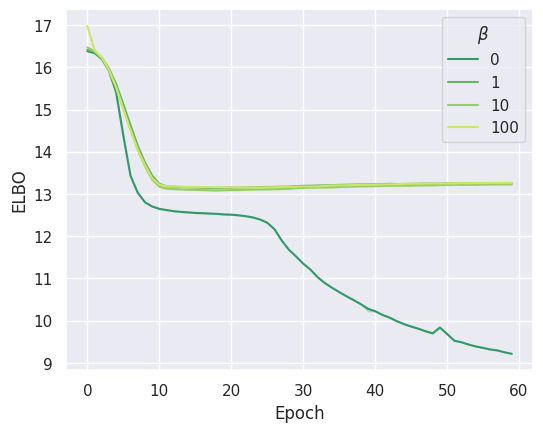
\includegraphics[width=.9\linewidth]{graphs/plots/beta_loss_fb.png}
      \caption{FB15K-237}
      \label{fig5:betafb}
    \end{subfigure}%
    \begin{subfigure}{.5\textwidth}
      \centering
      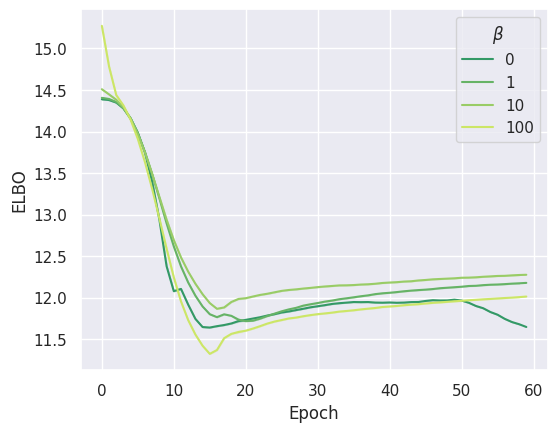
\includegraphics[width=.9\linewidth]{graphs/plots/beta_loss_wn.png}
      \caption{WN18RR}
      \label{fig5:betawn}
    \end{subfigure}
    \caption{Validation loss for RGVAE with $\beta \in [0,1,10,100]$ trained on each dataset.}
    \label{fig5:beta}
\end{figure}


Figure \ref{fig5:beta} shows the validation ELBO for the different $\beta$ values and for both datasets. We notice two interesting outcomes.  

\begin{itemize}
    \item For $\beta = 0$ converges further than the rest.
    \item The remaining values behave quase identical with $\beta = 100$ performing slightly better. 
\end{itemize}

Since setting $\beta = 0$ would undermine our hypothesis of evaluating variational model, we chose $\beta = 100$ as default for the following experiments. This also compares with the $\beta$ values proposed by Higgins in \cite{higgins_beta-vae_2016} to achieve a factorization of the latent space.

Especially on the FB15k-237 dataset the $\beta = 0$ configuration converges to a much lower ELBO. Thus, we have the trained models perform link-prediction on a $1\%$ subset of the validation set. Figure \ref{fig5:betafbmrr} indicates an inverse correlation between the ELBO and the MRR score. 

\begin{figure}[H]
    \centering
      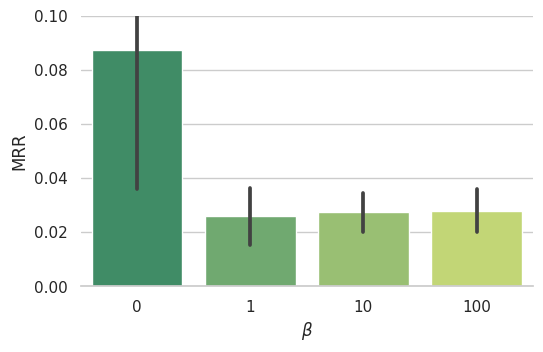
\includegraphics[width=.45\textwidth]{graphs/plots/beta_mrr_fb.png}
      \caption{MRR scores for different $\beta$ values on the dataset FB15k-237.}
      \label{fig5:betafbmrr}
\end{figure}

Barplot IN APPENDIX  

% d_z
Experiments on the impact of $d_z$ on the ELBO show little improvement for $10<d_z<100$ and from $100<d_z<1000$ insignificant to no improvement. Thus, we chose $d_z=100$ as default for our experiments.


% d_h did not influcence
Lastly, we evaluate the models hidden dimensions $d_h$ and its influence on the ELBO and the (subset)MRR. We compare between $d_h\in [256, 512, 1024, 2048]$, while the lowest configuration performs slightly worse on the ELBO, there is no significant difference between the remaining three configurations. Considering the models parameter count we chose the $d_h=512$ as default.


\subsection{Link Prediction}


 We now get to the main experiment of this thesis. The results of this experiment will show if the RGVAE architecture is suitable for link prediction and in first place, if it is able to grasp the underlying KG semantics at least significantly better than random by differentiating between real and corrupted triples. First we evaluate the performance of the RGVAE on this experiment, comparing both encoder versions. Then we investigate the influence of the variational inference by comparing the variational and original versions of DistMult on link prediction.
 
 \subsubsection{RGVAE}

 At this point we bring in the convolutional variation of our model, which we will denote as RGCVAE. The experiments reveal if the convolutional architecture holds an advantage compared to the simple MLP baseline. Further a randomly initiated and untrained RGVAE is used as control model.
 
 Due to its sparse graph computation, the RGVAE takes about 7 days to evaluate link prediction on the full test set and even 3 days when prediction tasks run parallel on a node of $4$ Nvidia Titan RX 25GB GPUs. Since the exemplary link prediction during experimenting with different hyperparameter already gave us an idea of the mediocre performance of our model, we chose to spare computation time and power by running link prediction on a randomly drawn one-third of the complete test set. Each run is repeated three times using a different random seed.

The results are visualized in figure \ref{fig5:lp_final}. We chose a visualization over a table, to emphasize our observations, and for the mentioned limitation of the test set, which makes these results not suitable for academically valid comparisons. Note that the figures are scales and to a range $[0,10]$ while all metrics have a maximum of $1$.

Comparing a MRR of $0.08$ to the DistMult score or $0.4$ our model does not perform competitively on link prediction tasks.

% Better than random?? I hope so.

Graph convolutions do not yield an advantage over the basemodel. In fact, the RGVAE with convolutions even scores slightly worse. 

%  FOR Conclusion: this might be because of the implementation of stacking the matrices.
The model scores about three times better on the FB15k-237 dataset than on WN18RR. FB15k-237 is a richer dataset with more triples and and a more balanced ratio of entities to relations. WN18RR operates on only 18 relations, what makes the relation most crucial when completing a triple. The architecture of the RGVAE puts twice the emphasis entities, described by the adjacency and the node feature matrices, while the relation is only represented by the overly sparse edge attribute matrix. Thus, we could conclude that our model learns to predict based on the hidden types and topics of the entities. All possible conclusions for this are discussed in \ref{sec:discus}. Relevant for this section is solely, that we chose the FB15k-237 dataset to investigate further, how well the RGVAE's grasps the underlying entity types and triple topics.   

%  REASON: fb has more relations, is a more complete KG. wn only 12 relations and more entities. Model emphasizes entities (adj and node features), relations may be less relevant, wn is more about the relation (same/ not the same). This indicates that our model grasps the hidden types and topics of the FB entities.


 \begin{figure}[H]
  \centering
  \begin{subfigure}{.5\textwidth}
    \left
    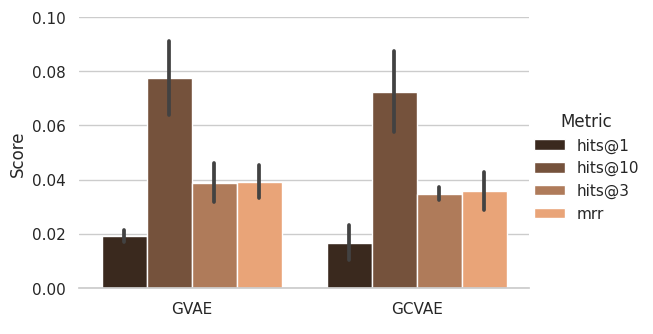
\includegraphics[height=.5\textwidth, keepaspectratio]{graphs/plots/lp_fb.png}
    \caption{FB15K-237}
    \label{fig5:lpfb}
  \end{subfigure}%
  \begin{subfigure}{.5\textwidth}
    \right
    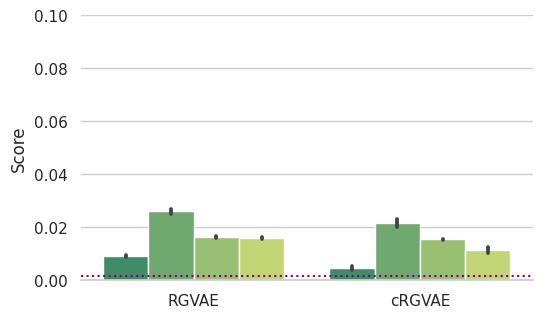
\includegraphics[height=.5\textwidth]{graphs/plots/lp_wn_wol.png}
    \caption{WN18RR}
    \label{fig5:lpwn}
  \end{subfigure}
  \caption{Link prediction results in MRR, Hits@1, Hits@3 and Hits@10 for RGVAE and RGCVAE trained on the full trainset of each dataset.}
  \label{fig5:lp_final}
\end{figure}

% TODO add random!!!

% Compare with vs without convolution 
% We use negative elbo as scoring function. Since elbo is aimed to be reduced and LP scores are higher better.

% We try with and without permutation

% We try the model as encoder only NO

% We use 1/3 of the test set only, randomly drawn. Run 3 times?
% Final models only 60 epochs


\subsubsection{Impact of Variational Inference and Gaussian prior}

In order to explain the poor performance of the RGVAE on the task of link prediction, we investigate the impact of the variational inference. Since the RGVAE with relaxed latent space, meaning less variance, indicated higher scores than the version with Gaussian prior, we examine the two variants by means of embedding models. The original DistMult model with optimized parameter serves as control model, while we compare it to the VDistmult, described in section \ref{ssec4:vdistm}, learning the full ELBO versus learning only on the reconstruction loss. By not including the regularization term in the loss the model is no longer bound to the Gaussian prior, which results in a relaxation of the latent space.

We train the three models for $300$ epochs solely on the FB15k-237 dataset and evaluate MRR, Hits@$1$, Hits@$3$ and Hits@$10$. Table \ref{tab5:VarDistM} shows the mean scores with $\mu \pm \sigma$ of three runs per model. Note that the exponent on $\sigma$ holds for the whole term. We can clearly see that both variational versions of the DistMult perform significantly worse than the original model. Learning on the full elbo or only the reconstruction loss does not seem to influence the scores in this setting. This indicates, that the models performance on link prediction suffers from using variational inference.

In the last row we show the results of the RGVAE with relaxed latent space. This model was trained with $\beta=0$ thus not constraining the latent space on a Gaussian prior. The model outperforms the versions with hyperparameter choice $\beta>0$ and scores the closest to the DistMult model. The impact of $\beta$ shows in the regularization, which we tracked separately. The maximum values of$D_{K L}$ during the experiment are 

\begin{equation}
  \begin{align}
    D_{reg} &= \beta D_{K L}\left(q_{\phi}\left(\mathbf{z} \mid G\right) \| p_{\theta}(\mathbf{z})\right) \\
    \max_{\beta = 0} D_{K L} &= 3506 \\
    \max_{\beta = 100} D_{K L} &= 0.0154
  \end{align}
  \label{eq5:KLdifferentBeta}
\end{equation}


While the results of the relaxed RGVAE might seem promising, Distmult is a much simpler and faster link predictor, thus we do not see a justification to keep researching on the RGVAE for this task. Note that due to the high computation cost of the RGVAE we only run the experiment once on the full dataset.

% TODO: Answer question:Link prediction with control model:

% Trained for 300 epochs

% We see that the variational part messes everything up.

% Table:
% MRR + Hits@all + Loss

\begin{table}[H]
  \centering
      \begin{tabular}{|l|l|l|l|l|}
      \hline
      \rowcolor[HTML]{EFEFEF}
      \multicolumn{1}{|c}{\textsc{Model}} & \multicolumn{1}{c}{\textsc{MRR}} & \multicolumn{1}{c}{\textsc{Hits@$1$}} & \multicolumn{1}{c}{\textsc{Hits@$3$}} & \multicolumn{1}{c|}{\textsc{Hits@$3$}} \\\hline
      DistMult     & \multicolumn{1}{c|}{$0.2854\pm 0.0025$} & \multicolumn{1}{c|}{$0.2\pm 0.001$} & \multicolumn{1}{c|}{$0.3149\pm 0.0038$} & \multicolumn{1}{c|}{$0.4512\pm 0.0053$}  \\
      VDistMult   & \multicolumn{1}{c|}{$0.517\pm 0.0197e^{-3}$} & \multicolumn{1}{c|}{$0.2442\pm 0.1994e^{-4}$} & \multicolumn{1}{c|}{$0.8145 \pm 0.3049e^{-4}$} & \multicolumn{1}{c|}{$0.399\pm 0.0576e^{-3}$} \\
      VDistMult w/ ELBO   & \multicolumn{1}{c|}{$0.6397\pm 0.0357e^{-3}$} & \multicolumn{1}{c|}{$0.57\pm 0.3046e^{-4}$} & \multicolumn{1}{c|}{$0.1547\pm 0.1023e^{-3}$} & \multicolumn{1}{c|}{$0.6351\pm 0.1992e^{-4}$} \\
      RGVAE w/o ELBO   & \multicolumn{1}{c|}{$0.1412$} & \multicolumn{1}{c|}{$0.0981$} & \multicolumn{1}{c|}{$0.1494$} & \multicolumn{1}{c|}{$0.2275$} \\
      \hline
      \end{tabular}
      \caption{Link prediction scores of DistMult and RGVAE versions on the FB15k-237 dataset.}
      \label{tab5:VarDistM}
  \end{table}


\subsection{Impact of permutation}
% Check if adj matrix adheres to edge attribute matrix.

Furthermore we examine the influence of the permutation invariant loss function described in \ref{ssec4:loss}. During training and subset link prediction no significant difference was observed between the RGVAE with versus without matching target and prediction graph. Yet, two observations draw our attention, namely:

\begin{itemize}
  \item The amount of nodes permuted per batch converges during training from $100$\% to exactly $60$%.
  \item The RGVAE with permutation invariant loss function learns to predict many variations of adjacency matrix while the standard model predicts similar to the target.
\end{itemize}

The first point indicates that the model learns a set of adjacency matrices, which can be permuted to match the target while optimizations the loss. Note that the generated matrix representation of the triples either has only one edge on the right upper index $A_{0,n}$ or, in the rare case of self-loops in $A_{0,0}$. The number of nodes per graph for these observations is set to $n=2$. Curiosity remains why the model converges to steadily permute $\frac{3}{5}$ of the prediction.
Secondly, we see that even when converged, the model predicts variations od the adjacency matrix very different to the target. The most common is a single edge on $A_{n,0}$ and on $A_{n,n}$. Less common and with lack of explanation are the predictions of an empty, or multi edge adjacency matrix. In contrast to this and as expected, the RGVAE with the standard loss function learns to solely predict edges on $A_{0.0}$. 
Finally we will analyze the impact of permutation invariance on the experiment of syntax coherence in section \ref{ssec5:syntax}.


% Permutation starts at $100\%$ at the beginning of training and converges to $60\%$.

% Model without predicts adj node always in the upper right just as the target. Model with predicts much more variations of adjacency.

% Graph of permutation during training.
% loss with vs without 

\begin{figure}
  \caption{(a) Validation loss RGVAE with vs. w/o permutation invariant loss function. (b) Percentage of permuted nodes during training.}
  \label{fig5:permInv}
\end{figure}

\subsection{Interpolate Latent Space}

Inspired by the popular results of Higgins, who featurized each latent dimension on a facial features of the FACES dataset \cite{ebner_facesdatabase_2010}. The VAE generates faces controlling feature such as age, gender and emotions by manipulating single latent dimensions \cite{higgins_beta-vae_2016}.  We run this experiment with the RGVAE on the FB15k-237 dataset, using two different interpolation methods. The latent dimension for this experiment is set to $d_{z}=10$ in order to analyze each dimension separately and the interpolation is linear with a step count of $10$.

The first experiment is linear interpolating between two triples. Therefor two valid triples from the train set are encoded into their latent representation. We chose the two semantically related triples triples to analyze if the linear movement in latent space correlates with an obvious semantic feature. 

\begin{center}
  \texttt{[['/m/02mjmr Barack Obama'], ['/people/person/place\_of\_birth'], ['/m/02hrh0\_	Honolulu']]}
  \texttt{[['/m/058w5 Michelangelo'], ['/people/deceased\_person/place\_of\_death'], ['/m/06c62	Rome']]}
\end{center}


% TODO present the results and link to appendix

\begin{table}[H]
  \centering
  \begin{tabular}{|c|}
  \hline
  \rowcolor[HTML]{EFEFEF} 
  \textsc{RGVAE permutation}\\ \hline
  \texttt{[[France] [/base/petbreeds/city\_with\_dogs/top\_breeds] [Imperial Japanese Army]]}\\
  \texttt{[[Cree Summer] [/tv/tv\_program/program\_creator] [David Chase]]}\\
  \texttt{[[Guitar] [/business/business\_operation/assets] [Paramount Vantage]]}\\
  \texttt{[[Democratic Party] [/music/genre/artists] [Howard Hawks]]}\\
  \texttt{[[Roy Haynes] [/people/person/spouse\_s] [The Portrait of a Lady]]}\\
  \texttt{[[Cleveland Browns] [/film/actor/dubbing\_performances] [David Milch]]}\\
  \texttt{[[Jay-Z] [/film/special\_film\_performance\_type/film\_performance\_type] [Ashley Tisdale]]}\\
  \texttt{[[Phoenix Suns] [/film/film/dubbing\_performances] [Lynn]]}\\
  \texttt{[[James E. Sullivan Award] [/organization/organization/child] [Giant Records]]}\\
  \texttt{[[Boston United F.C.] [/soccer/football\_player/current\_team] [Kensal Green Cemetery]]}\\  
  \hline
  \end{tabular}
\caption{Latent space interpolation between two triples in $10$ steps.}
\label{tab5:ipbtw2}
\end{table}
% Obama triple is not reproduced, not even close.

For the second experiment, we interpolate each latent dimension isolated in a $95\%$ confidence interval of the Standard Gaussian distribution. Starting with the encoded representation of the Obama triple, we incrementally add $z_{i} += -1.96 + j \times s$ with $s = \frac{1.96 * 2}{n_s-1}$ for the number of steps $n_s = 10$. Due to the size of the tables representing the interpolations and the low value they add to the presentation of this work, the result of this experiments can be found in the appendix.


% Further we go ahead and test what happens if we modify one latent dimension at a time with $d_z = 10$ of a triple. TABLE: (s,r,o), x axis dims, y axis steps. $95\%$ Gaussian confidence 

% Can the model assign logical features to latent dimensions?


\subsection{Syntax coherence}
\label{ssec5:syntax}

On closed-world schema-based KGs the approach for testing the validity of a new triple is to add it to the existing KG and run a onthology reasoner on it. A inconsistency in the KG will appear as \texttt{null}-Class, but only if an axiom is violated. This approach works only for fully constrained KGs and is not scalable, since the reasoner recursively checks evey triple for every axiom. Thus, we present an alternative and improvised way to estimate the validity of generated triples.

The FB15k-237 is a subset from the FreeBase KG \cite{bollacker_freebase_2008}, thus, even thought they are not part of the dataset, - entities have type properties in their original Freebase representation. 
Querying the last official Freebase dump, we get the types for each entity in the FB15k-237 dataset, With exception of $8$ entities, which could not be found in the query.

Our approach is to randomly generate triples, from signals randomly drawn from a Standard Gaussian distribution. Then to filter those triples on predicates which contain the type \textit{people}, which is within the top 10 most common Freebase types. We differentiate between base-class types subclass types, both can contain the word \textit{people}. The entity \texttt{['/m/02mjmr Barack Obama']} has between many others the type \texttt{[/people/measured\_person]}. Here the base class is \textit{people} and the subclass \textit{measured\_person}. We could filter directly on subclasses, but we chose to give our model more creative freedom and filter for \textit{people} in the full set of types. Using this choice, the generated triples are scored on logic rather than facts. E.g. any person can hypothetically the a \textit{measured\_person}, understanding this implies semantical reasoning, while differentiating between which person is and is not a \textit{measured\_person} implies contextual knowledge. Thus, we use the base type \textit{people} to validate triples.
Furthermore the relations are inconsistent in their notation, partly not only having a head type constrain. Thus, we check only the head entity for the key type. 

\begin{itemize}
  \item From $14541$ entities, $5283$ contain the keyword people, or $36.332$\%.
  \item From $237$ predicates, $25$ contain the keyword people, or $10.549$\%.
  \item From $310116$ triples, $47354$ contain the a predicate keyword people, or $15.269$\%.
\end{itemize}

Considering these facts, we calculate the marginal probability of guessing a head entity $s$ of type \textit{people}, given a triple which contains the type \textit{people}. Without prior knowledge $p(s_{p})$ and $p(r_{p})$ are conditionally independent. The probability is calculated as:

\begin{equation}
  p(s_{p} \mid r_{p}) &= p(s_{p}) = 0.3633
  \label{eq5:randomValid}
\end{equation}

For this experiment we generate triples until $10e^5$ contain the key type. Those filtered triples are validated on the type of the head entity and compared to the full dataset for novelty. Here we again compare the performance between the RGVAE with the two different encoder architectures. Furthermore the models are trained both with regular and permutation invariant loss function. Lastly, the experiments are repeated for sampling the latent signal from $\mathcal{N}(0,1)$ and for sampling from $\mathcal{N}(0,2)$.  We average the accuracy of three runs of generating a valid triple and of this triple being unseen in the dataset. The results for valid triples are shown in figure \ref{fig5:syntax}. The dotted horizontal line indicates the random probability of generating a valid triple, calculated in equation \ref{eq5:randomValid} and $\sigma^2_1$ and $\sigma^2_2$ denote the variance for the different latent space distributions. 



\begin{figure}[H]
  \centering
  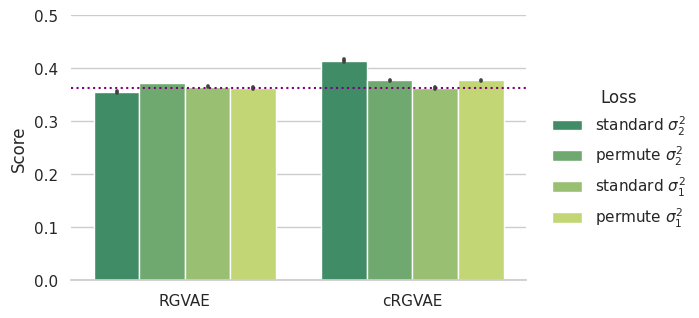
\includegraphics[height=.25\textwidth, keepaspectratio]{graphs/plots/kg_all.png}
  \caption{Accuracy of generating valid triples.}
  \label{fig5:syntax}
\end{figure}

To our disappointment the model does not perform significantly better than random. Neither the choice loss function nor the doubled variance show a correlation with the accuracy. The only configuration standing out is the RGVAE with convolutional encoder, standard loss function and $\sigma^2=2$, scoring $4$\% higher than random. From all valid generated triples $100\pm 0.001$\% are new and unseen in the dataset. Coming back to \texttt{['/m/02mjmr Barack Obama']}, we filter the unseen triples fo the first three appearances of this entity. These are displayed in table \ref{tab5:genTriples} for every variation of the RGVAE and in the same order as in figure \ref{fig5:syntax} 



\begin{table}[H]
  \begin{tabular}{|c|}
  \hline
  \rowcolor[HTML]{EFEFEF} 
  \textsc{RGVAE standard} $\sigma_2^2$\\ \hline
  \texttt{[[Barack Obama]	[/people/person/places\_lived./people/place\_lived/location]	[Casablanca]]}\\
  \texttt{[[Barack Obama]	[/people/person/place\_of\_birth]	[Sarah Silverman]]}\\
  \texttt{[[Barack Obama]	[/people/person/place\_of\_birth]	[The League of Extraordinary Gentlemen]]}\\ \hline
  \rowcolor[HTML]{EFEFEF} 
  \textsc{RGVAE permuted} $\sigma_2^2$\\ \hline
  \texttt{[[Barack Obama]	[/people/ethnicity/geographic\_distribution]	[End of Watch]]}\\
  \texttt{[[Barack Obama]	[/people/profession/specialization\_of]	[Montgomery County]]}\\
  \texttt{[[Barack Obama]	[/people/cause\_of\_death/people]	[WWE Superstars]]}\\ \hline
  \rowcolor[HTML]{EFEFEF} 
  \textsc{RGVAE standard} $\sigma_1^2$\\ \hline
  \texttt{[[Barack Obama]	[/people/person/place\_of\_birth]	[Academy Award for Best Sound Editing]]}\\
  \texttt{[[Barack Obama]	[/people/person/places\_lived./people/place\_lived/location]	[Stan Lee]]}\\
  \texttt{[[Barack Obama]	[/people/person/place\_of\_birth]	[Multiple sclerosis]]}\\ \hline
  \rowcolor[HTML]{EFEFEF} 
  \textsc{RGVAE permuted} $\sigma_1^2$\\ \hline
  \texttt{[[James Brolin]	[/people/person/places\_lived./people/place\_lived/location]	[Barack Obama]]}\\
  \texttt{[[Barack Obama]	[/people/person/spouse\_s./people/marriage/location]	[D.C. United]]}\\
  \texttt{[[Jim Sheridan]	[/people/person/religion]	[Barack Obama]]}\\ \hline
  \rowcolor[HTML]{EFEFEF} 
  \textsc{cRGVAE standard} $\sigma_2^2$\\ \hline
  \texttt{}\\
  \texttt{None}\\
  \texttt{}\\ \hline
  \rowcolor[HTML]{EFEFEF} 
  \textsc{cRGVAE permuted} $\sigma_2^2$\\ \hline
  \texttt{[[Pinto Colvig]	[/people/deceased\_person/place\_of\_burial]	[Barack Obama]]}\\
  \texttt{[[Helena Bonham Carter]	[/people/person/gender]	[Barack Obama]]}\\
  \texttt{[[John Buscema]	[/people/person/spouse\_s./people/marriage/spouse]	[Barack Obama]]}\\ \hline
  \rowcolor[HTML]{EFEFEF} 
  \textsc{cRGVAE standard} $\sigma_1^2$\\ \hline
  \texttt{[[Suhasini Ratnam]	[/people/person/sibling\_s./people/sibling\_relationship]	[Barack Obama]]}\\
  \texttt{[[Barack Obama]	[/people/person/gender]	[Deva]]}\\
  \texttt{[[Barack Obama]	[/people/person/sibling\_s./people/sibling\_relationship]	[Niagara Falls]]}\\ \hline
  \rowcolor[HTML]{EFEFEF} 
  \textsc{cRGVAE permuted} $\sigma_1^2$\\ \hline
  \texttt{[[Jonathan Rhys Meyers]	[/people/person/nationality]	[Barack Obama]]}\\
  \texttt{[[Barack Obama]	[/people/person/sibling\_s./people/sibling\_relationship]	[Motherwell F.C.]]}\\
  \texttt{[[Pinto Colvig]	[/people/deceased\_person/place\_of\_burial]	[Barack Obama]]}\\ \hline
  \end{tabular}
\caption{Generated and unseen knowledge.}
\label{tab5:genTriples}
\end{table}


The generated triples confirm the accuracy results. With exception of the triple 
\begin{center}
  \texttt{[[Barack Obama]	[/people/person/places\_lived./people/place\_lived/location]	[Casablanca]]} 
\end{center}

all remaining triples violate common sense logic. The RGVAE does not differentiate between the types gender, location, movie, person or medicine. It even goes so far to state that Obama was born in \texttt{[Multiple sclerosis]}. While this might sound funny it also clearly indicates, that our model did not learn the underlying semantics of this real world KG.

While investigating the model and the generated triple set, we notice two outcomes. Neither the augmentation of the variance nor the enabling of the permutation invariance has an impact on either of the model with two encoder versions. The regularization loss converges during training to zero, meaning that the model learns a latent representation of the dataset as  nearly perfect Standard Gaussian distribution. Yet, even when sampling latent signal from the exact same distribution, we notice that each model repeatedly predicts combinations of a small subset of entities and relations, e.g. the RGVAE version which did not predict the Obama entity once in a total of $111583$ valid triples. This also aligns with the interpolation results, where we observed a static relation for the full gridsearch of the latent space. If we look at the gradient and parameter values $\phi$ and$\theta$ of the MLP encoder and decoder, we see a much higher variance and gradients for $\phi$. The decoder shows higher values and variance for a small subset of neighboring parameter, while the remaining parameters converge to a very similar and low value. This indicates that the encoder learns very well to represent each different triple as Standard Gaussian latent representation. The decoder MLP on the opposite seems to to ignore most of this representation by assigning vanishing values to the connected parameters. Intuitively it seems that the decoder learns to interpret the part of the latent representation corresponding to the adjacency matrix and minimizes as well as stabilizes the loss of the edge and node attribute matrix by uniformly distributing their probability. This leads to the decoder reconstructing edge and node attribute randomly. Further, depending on the values of $\theta$ when the model finishes learning, the decoder will keep predicting the same subset of entities and relation independent of the latent signal $z$. If we look at the flattened representation of our input graph, we see that the part representing the adjacency matrix is way shorter and has a tractable mean of $\frac{1}{4}$ while the mean for the edge and node attribute matrices are $\frac{1}{{4 \times 1345}}$ and $\frac{1}{14951}$. The problem of a our decoder partly ignoring the latent input and potential solutions are discussed further in section \ref{ssec7:collapse}. 


\subsubsection{Delta Correction}
\label{ssec5:delta}


% Explain quick delta implementation 

% Explain new experiments

% show interesting interpolation

% show parameters if different

\begin{figure}[H]
  \centering
    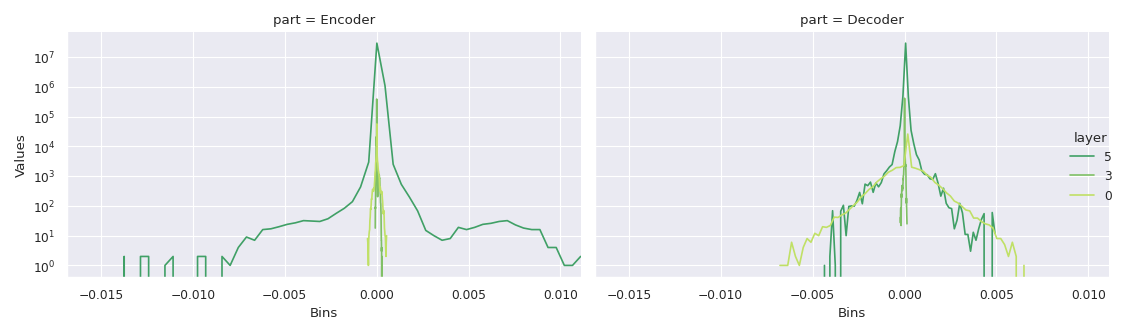
\includegraphics[width=\textwidth]{data/ip/GVAE_p1_delta_encoder.png}
    \caption{MRR scores for different $\beta$ values on the dataset FB15k-237.}
    \label{fig5:deltaParams}
\end{figure}


\begin{figure}[H]
  \centering
    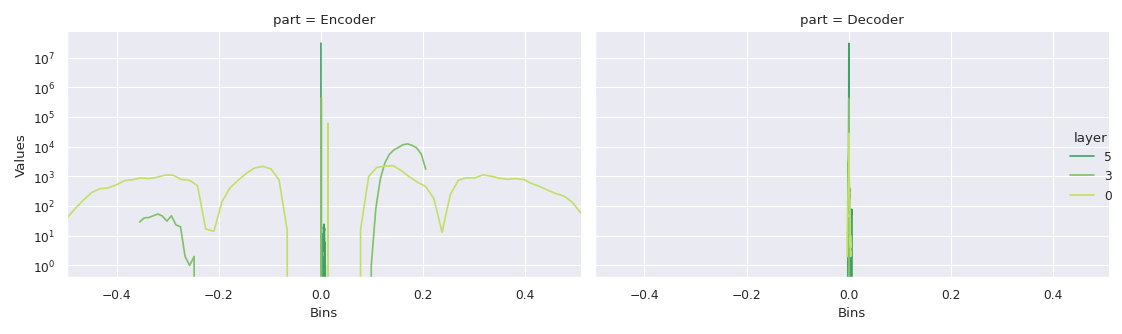
\includegraphics[width=\textwidth]{data/ip/GVAE_p1_encoder.png}
    \caption{MRR scores for different $\beta$ values on the dataset FB15k-237.}
    \label{fig5:normParams}
\end{figure}


% \section{Results}
% Fabulous results only!

\section{Discussion \& Future Work}

% TODO compare to molecules - point out differences

In this final chapter, we will discuss our results from different experiments, emphasizing the comparison to Simonovsky's work on molecule generation. The fact, that we did not achieve Similarly successful results does not hinder us from analyzing the responsible factors and causalities. Despite the nature of our results we are happy to propose possible solutions and while being of the opinion that questions are often more interesting than answers, we will question the value of these solutions for further research.

\subsection{Experiment Take-away}

% Well well well
% We did link prediction because it is the most common experiment in this field

%  We see loss converges perfectly 
The first relevant observation made is the lower ELBO score to which the RGVAE converges when using $\beta=0$, meaning it is only trained on the reconstruction loss.
We tested the assumption that the model performs better without regularization term. This leads to the assumption that the RGVAE performs better better without prior constrain, yet a fully unconstrained VAE, defies the its purpose when it comes to disentangling the latent space and sampling.
The tuned RGVAE shows poor results on the task of link prediction, with slightly worse scores for the convolutional encoder. In order to find the isolate the causalities, we experiment further on link prediction with two variational version of DistMult learning on the full ELBO and only on the reconstruction loss. Both models scored equally bad compared to the original model, indicating that DistMult and embedding based link predictors in general are not complex enough for variational inference. Following our prior assumption we added the unconstrained RGVAE to this comparison, which led to significantly higher scored than the all versions of the tuned RGVAE and the variation DistMult. Yet, the scores were not competitive with state of the art link predictors of with much lower parameter count, thus we do not recommend further researching in the direction of VAE as link predictor.

The graph matching loss function does not seem to have any impact on the link prediction results, yet we cannot draw a conclusion here since since the poor performance is linked to a different causality which might impede the graph matching from adding value. To measure the percentage of permutation we adopt Simonovsky's method of averaging the identity of permutation matrix $X$, which is invariant for permutation equivalent nodes. We see that during training the permutation rate converges to $60$\%.

Comparison of the two datasets, showed a better performance on the FB15K-237 dataset. While both datasets are real-world KGs, WN18RR is composed of synsets with vast discrepancy between the relation and entity count, resulting in a lower chance of generating a valid triple. Thus, we decided to continue the interpolation and graph generation experiments only on the FB15k-237 dataset. 

For the last two experiments we trained the RGVAE with $d_z=10$ for better disentanglement and analysis of each latent dimension.
The interpolation experiment between two triples reveals that the RGVAE in all versions fails to reconstruct the start and end triple. We notice an influence of the graph matching loss, namely the model predicting constantly the same relation versus the standard loss, where the model predicts randomly from a subset of triples. Same can be said for the predicted entities, which are drawn from a subset of what seems to be the most frequent occurrences in the dataset. Empirically we can say that the prediction has little prior conditioning on the latent signal.

These last experiment is designed and evaluated in a similar fashion as Simonovsky did to generate valid molecular graphs. We interpolate the full latent space for $-\sigma^2 < z < \sigma$ and $-2\sigma^2 < z < 2\sigma$. Based on our proposed validation criteria, the RGVAE generated the same rate of valid triples as random. We observe further independence between the decoder and the latent signal. This slightly compares with Simonovsky's result where the generated valid triples had a variance of only $10$\%.
% Interpolation
%  like molecules


% Why does graph matching change that? 
% Higher dimension of freedom when generating graphs using Graph matching.

% All valid generated triples are unseen in both train and test set. 

% Simonovsky also reports low variance of valid triples 10\%

\subsection{Research Answer}

% Answer it right!

% How successful is a VAE in representation learning on real world KG compared to molecule graph data and what is the impact of each major hyperparameter?

%  Overall
To answer the initial research question we will first summarize the influence of the main hyperparameter.

%  Convolutions
A convolutional encoder does not seem to contribute to the performance of the RGVAE. This could be caused by the simple implementation of using node and edge attributes both as feature matrix, or be due to the decoder issue, explained in \ref{ssec7:collapse}, that the prediction is independent of the encoding. 

%  graph matching
Graph matching does have a noticeable impact. The model expresses more creative freedom when predicting the adjacency. Especially for experiments with larger subgraphs we recomend to keep investing in this method.

%  Prior, stochasticity
Variational inference is part of the VAE and allows disentanglement of the latent space, thus, even considering that the unconstrained model scored better, we recommend keeping the VAE structure. Instead of the full stochastic module, we assume the Standard Gaussian prior to be the reason behind the poor representation and we recommend comparing alternative prior constrains.

Overall we can answer the research question:

\begin{center}
    \textit{The RGVAE failed in representation learning of real-world KG due to the Standard Gaussian latent space prior.}
\end{center}

Yet, metaphorically, this is not the end of the book, but rather the beginning of a new chapter. In the remaining part of this discussion we analyze the underlying problem of the RGVAE and propose a variety of solutions.


\subsection{Decoder Collapse}
\label{ssec7:collapse}

%  what is decoder collapse
To introduce the main part of our conclusion we explain a phenomenon observed when training GANs. A GAN is yet another generative model which based on its potential to generate high resolution images, has drawn much attention in recent years. It consists of a generator, who's task it is to decode a latent signal to a an image, and a discriminator, which given the fake image and the real data has to distinguish between them. Training of GANs is unstable and one of the major problem which occur is \textit{mode collape}. The generator learns to fool the discriminator by generating only a single mode with high precision such that the discriminator classifies it was real image.

While VAEs cannot suffer from mode collapse, because they backpropagate over the predicted distributions of all modes, it has a related phenomenon. \textit{Decoder collapse} occurs when the decoder has enough capacity to choose not to consider the latent signal and instead stores the information to reconstruct the data's distribution partly or solely in its parameters. This means that the generated data is not conditioned on the latent signal anymore. The cause of this problem is found in the regularization term $D_{K L}\left(q_{{\phi}}\left(\mathbf{z} \mid \mathbf{x}\right) \| p_{{\theta}}(\mathbf{z})\right)$, more specifically in the constrain on a standard Gaussian prior. The multidimensional encoding of $d_z>1$ the approximated posterior is a mixture of Gaussians, which can only match the multivariant Normal distribution, in the case of all $\mathbf{\mu}_z=0$ and $\Sigma^2_z=\mathbb{I}$, what also implies that no information is encoded. Thus, the VAE has to decide if storing information in the latent vector is necessary to model the dataset distribution $p(x)$. If the penalty for altering the latent Normal distribution outweighs the benefits of the additional information towards the reconstruction loss, the VAE will chose for \textit{decoder collapse}. 

%  Cite https://towardsdatascience.com/with-great-power-comes-poor-latent-codes-representation-learning-in-vaes-pt-2-57403690e92b

% when we use a decoder with so much capacity that it chooses to not store information in the latent code at all, a result that leaves important information about our distribution locked up in decoder parameters, rather than neatly extracted as an internal representation.

% the network will only choose to make its z value informative if doing so is necessary to model the full data distribution, p(x). Otherwise, the penalty it suffers for using an informative z will typically outweigh the individual-image accuracy benefit it gets from using it.

% analyze results of interpolation and generation
Exactly this phenomenon can be observed in the triple interpolation and generation experiments. The RGVAE converges rapidly during training, minimizing the reconstruction loss close to zero. This falsely indicates that the model has learned to reproduce the data. Yet, when sampling using only the decoder, the generated triples repeat combinations of a subset of entities and relations which are more frequent in the dataset. During interpolation of the latent space, the model predicts steadily the same relation. Subject and object seem rather randomly drawn, showing little impact while traversing each single latent dimension. The adjacent matrix >>><<<

The last experiment confirms the obvious. The syntax adherence of the different model variations does not differ from random sampling. Further we again notice the predominance of the more frequent data.


% For link prediction this means that the reconstruction loss is not helpful at all. 
Projecting this finding on the link prediction experiment, we question, why the model scored better than random. Possible reasons are for once, that the encoder learned to encode the dataset close to a Normal distribution, but when encountering unseen triples, the mean and variance of the encoding vary. A second reason is, the every triple in the testset is corrupted in all possible combinations, including the less frequent entities. The collapsed decoder subsequently keeps generating frequent triples, thus the reconstruction loss between a less frequent combination of entities and the collapsed prediction will be higher than for a frequent combination. Therefore the model learns score the real triple higher but for the wrong reason. The RGVAE with $\beta = 0$ and therefore unconstrained on the Standard Gaussian prior shows the best results between the different model settings. We can assume that the model learns a latent representation for subject and object. Despite this improvement, is it probable that the decoder still collapses on the reconstruction of the relation index, which explains the remaining scoring gap to the much simpler DistMult model.


\subsection{VAE surgery}
\label{ssec7:solutions}
% Propose solutions: Elbosurgery, adversial(WAE),  recurrent(lossy)

Similar problems in different fields have been encountered for generative VAE applications. While the author of this thesis whishes to have drawn these parallels earlier, all the proposed solutions imply a significant modification of the VanillaVAE, thus would not align with this work's research question. We present three approaches from different literature which tackle the VAE mode collapse in the filed of image and voice generation.

%  ELBO surgery
In a publication of Adobe Research and Google Brain, Hoffman and Johnson propose an elegant modification of the variational evidence lower bound \cite{hoffman2016elbo}. 
More specifically they change the VanillaVAE's regularization term, where instead of imposing a Standard Gaussian prior on the full latent distribution, the prior is imposed on the mixture of all single latent dimension, giving space for more expressive probability distributions such as truncated Gaussians. 

Further, a index-code mutual information term is added, intended to maximize the mutual information between every index of the observation and $z$. While the reconstruction term enforces to encode every feature of $x$ in a corresponding latent dimension, the  information term opposes this by maximizing the mutual information between all  $x_i$ and $z_i$. The information term compares compact to the reconstruction loss, yet it is enough to prevent decoder collapse. 

SHOULD WE WIRTE THE NEW LOSS OUT?


% Lossy Auto Encoder
Kingma et al. turn towards a autoregressive solution in their publication \cite{chen_variational_2017}. Their VAE model generates images recursive per pixel, each conditioned on previous point, using both RNN and RCN as decoder. Their solution to the decoder collapse is a normalizing flow, which predicts the encoder posterior $q_{\phi}(z \mid x)$. Besides not suffering from decoder collapse, this model can be set to discard irrelevant information in the data. As downside, the autoregressive nature causes slow image generation.


% Wasserstein or AAE
The last approach we present closes the circle to the introduction of this section. The paper \textit{Wasserstein Auto-Encoders} \cite{tolstikhin_wasserstein_2019} propose a combination between GAN and VAE. A model wich uses the VAE's encoder-decoder architecture but instead of the normal regularization term, the posterior distribution is learned and penalized by its Wasserstein distance tp the data distribution. This is in fact a generalization of the adversarial loss of generator and discriminator. Since our task of generating triples would benefit from a precise prediction, such as GANs achieve on image generation, we question, if employing adversarial loss also on the reconstruction term would yield better generation results in this field than the exact index-wise loss?

% Two different papers, same principle:

% Use GAN loss for VAE latent space distribution. Generator produces a distribution and discriminator tys to tell if its fake or true.

% Similar approach with Wasserstein distance as regularization loss. 


% Could we also usefully employ adversarial loss on the reconstruction part of the network (that is: have a discriminator try to tell apart input and reconstruction), to get away from the over-focus on exact detail reconstruction that comes with pixel-wise loss


% Remaining: Amortized Inference Regulation and Skip Connections 
Besides these three, numerous other approaches have been proposed. Worth mentioning because of their originality are the idea of adding skip-connections between latent space and the decoder's hidden layer \cite{dieng_avoiding_2019} as well as regularizing the amortized inference \cite{shu_amortized_2019}.  

% delta-VAE <--

% Regulation of the amortized inference.

% Skip connections between latent space and hidden layer of the decoder.



% Two layerVAE

\subsection{Future Work}

There are many avenues to follow for future work. Obviously the first step is to fix the collapsing decoder. The suggested solutions should be compared before making a choice, since none has yet been shown to work on KG VAEs.

Once the reconstruction of triples proved successful, we should look at the data, and question the representation. The adjacency matrix can be inferred from the edge attribute matrix and thus, is obsolete. Since it does not contain additional information, does the model perform worse without it? Approaching this thought from a different angle, we could leave the adjacency as it is and represent the node and edge indices as continuous number, as it is done for color scales of images. This would greatly reduce the number of parameters, but certainly also imply new challenges. Important in this context is that the adjacency is represented in sparse format since this the experiments on triples is but a proof of concept for larger subgraphs. 

We noticed the model worst flexibility for predicting the relation index. In the interpolation experiment it kept predicting the very same relation for the entire latent space. Also linked is the variance in number of edges, while the number of nodes is constant. Thus, we wonder if a setup of two VAEs, where the first one predicts the adjacency and node attributes and the second recurrent one, while conditioned on the predicted edges of the first VAE, predicts the edge attribute.

Finally and making use of the batch wise implementation of the max-pooling graph matching alorithm presented in this work, we suggest to explore a more efficient and \textit{intelligent} graph matching approach. Would it be possible drasically reduce complexity by training a neural network to predict the optimal permutation matrix based on target and prediction graph?
% with one of the presented solutions, starting with the simplest.

% Is the adjacency matrix even necessary? 

% Basing on the believe that further research will be fruitful, we recommend:

% \begin{itemize}
%     \item Smarter approach for graph matching, let a NN learn the best permutation given the targe and prediction
%     \item Two VAEs, first one-shot only the adjacency, second recurrent edgewise including entity and relation index.
%     \item Disentangle the latent space and condition on text
%     \item NF prior
% \end{itemize}

We hope to have given enough food for though for everyone willing to continue research in this field and look with excitement towards future findings.

\textbf{Happy New Year!}


\section*{Ideas}


The bigger picture of this thesis is to efficiently generate a representation of the information hold in plain text. This representation has the form of a knowledge graph and consists of subject-relation-object triples.
\\
\textbf{Challenges:}\\
\begin{itemize}
    \item What knowledge are we looking for?
    I would like the model to focus on the most important information. This could for example be topic specific.
    \item Another option would be to extract based on a query or point of interest.
    Especially if we build the KG incrementally we can use this input as starting point and recursively build from there. 
\end{itemize}


\subsection{Use Normalizing Flows}\label{idea:NF}

\begin{itemize}
    \item Is it possible to generate a graph from text using Normalizing flow (NF)?
    \item Can we train such a NF unsupervised, using the output distributions as loss function?
    \item NFs can build KG at once or incrementally.
No one is using it, could have a reason.
\end{itemize}

    
\subsection{Recurrent VAE}\label{idea:VAE}

\begin{itemize}
    \item Recursively generate graph using a Variational Auto Encoder.
    \item Use query as start node.
    \item expand graph on that node.
Thiviyan and others work on VAEs as well.
Seems an easier approach.
Can analyze the latent space.

\end{itemize}

The encoder decoder strategy has been applied successfully in many cases.
Bellis thesis about modeling a graph from images can be applied to text as well by changing the input to a text vector \cite{belli_image-conditioned_2019}. Note that this is a supervised method and would require a dataset of text labeld with resulting KGs. To the best of my knowledge this does not exist yet.
\\
Same holds for the contrastive world model by Kipf. If we input text vectors instead of an image the model could recognize different objects in the text as it does with pixels \cite{kipf_contrastive_2020}. Here the model is trained unsupervised using a loss over the energy function of the graph embedding space TransE \cite{bordes_translating_2013}. An open question is if this would work for our approach.
\\
A bit more abstract is the idea of the feedback recurrent VAE \cite{yang_feedback_2020} where sound signals are encoded and decoded. This could also be adopted to text for instance with one sentence at a time, or a fixed number of tokens. Here the text vector would be induced as the latent input to the decoder. This would mean finding an translation of the models latent space to the work embedding. The dataset would consist of positive and negative examples of resulting graphs over timesteps.
\\
While text can be easily vectorized by word embeddings like word2vec, the graph representation seems more tricky. A reasonable approach following Bellis example would be to output a coordinates vector for the nodes and an adjantency matrix for their relationships. Here one node at a time is outputted and the relation is conditioned on the number of previous nodes.
Alternatively we could make use of the graph embeddings RASCAL or TransE.
Lastly the question remains how to model the graph when the nodes need to be predefined. A subgraph of DBpedia could be a good starting point.

\section*{Open Issues}
A section where note will be made on open issus. These aissues are ment to be discussed with Peter or Thivyian and ultimatly solved. No open issues should remain at the end of November.


\subsection{Graph matching}

% NetworkX offers graph matching algorithms as do other repos. The drawback is that they are programmed for smaller graph such as molecule graphs with undirected edges and no edge atribues, or these attributes are not taken into account and only the structure is compared.
% My implementation of the max-pooling graph matching algorithm from \cite{simonovsky_graphvae_2018} return a $n\times n\times k\times k$ matrix with integer values ${0,2}$. Most probably something went wrong here since this makes little sense regarding interpretation.
% When graphs are compared with NetworkX using the greedy-matching or minimum distance, the similarity matrix is a $2\times 2$ matrix for comparing two graphs.
% My question is which sort of graph matching makes more sense for our usecase.
% Further I struggle to interprete the similarity matrix - is that my job tho? Maybe its just meant to be used in the loss function as described! 

Hungarian algorithm:
Should we assume the affinity matrix is a cost or a profit matrix. If we assume it is a cost matrix and n != k the algorithm returns an error while padding. If we assume it is a profit matrix and convert it to a profit matrix it can handle any dimension. The shortest path varies with both approaches.
Further I assume the shortest path is what we are looking for and mask these entries with 1 and the rest of the matrix with 0.

\printbibliography
\end{document}

% \bibliographystyle{unsrt} % We choose the "plain" reference style
% \bibliography{fullrefs} % Entries are in the "refs.bib" file

